% \documentclass{article} % For LaTeX2e
% \usepackage{iclr2025_conference,times}
\documentclass[11pt, a4paper, logo, copyright, gdm]{google}
\usepackage[authoryear, sort&compress, round]{natbib}
\usepackage{times}

% Optional math commands from https://github.com/goodfeli/dlbook_notation.

\usepackage{amsmath,amsfonts,bm}

\newcommand{\figleft}{{\em (Left)}}
\newcommand{\figcenter}{{\em (Center)}}
\newcommand{\figright}{{\em (Right)}}
\newcommand{\figtop}{{\em (Top)}}
\newcommand{\figbottom}{{\em (Bottom)}}
\newcommand{\captiona}{{\em (a)}}
\newcommand{\captionb}{{\em (b)}}
\newcommand{\captionc}{{\em (c)}}
\newcommand{\captiond}{{\em (d)}}

\newcommand{\newterm}[1]{{\bf #1}}


\def\figref#1{figure~\ref{#1}}
\def\Figref#1{Figure~\ref{#1}}
\def\twofigref#1#2{figures \ref{#1} and \ref{#2}}
\def\quadfigref#1#2#3#4{figures \ref{#1}, \ref{#2}, \ref{#3} and \ref{#4}}
\def\secref#1{section~\ref{#1}}
\def\Secref#1{Section~\ref{#1}}
\def\twosecrefs#1#2{sections \ref{#1} and \ref{#2}}
\def\secrefs#1#2#3{sections \ref{#1}, \ref{#2} and \ref{#3}}
\def\eqref#1{equation~\ref{#1}}
\def\Eqref#1{Equation~\ref{#1}}
\def\plaineqref#1{\ref{#1}}
\def\chapref#1{chapter~\ref{#1}}
\def\Chapref#1{Chapter~\ref{#1}}
\def\rangechapref#1#2{chapters\ref{#1}--\ref{#2}}
\def\algref#1{algorithm~\ref{#1}}
\def\Algref#1{Algorithm~\ref{#1}}
\def\twoalgref#1#2{algorithms \ref{#1} and \ref{#2}}
\def\Twoalgref#1#2{Algorithms \ref{#1} and \ref{#2}}
\def\partref#1{part~\ref{#1}}
\def\Partref#1{Part~\ref{#1}}
\def\twopartref#1#2{parts \ref{#1} and \ref{#2}}

\def\ceil#1{\lceil #1 \rceil}
\def\floor#1{\lfloor #1 \rfloor}
\def\1{\bm{1}}
\newcommand{\train}{\mathcal{D}}
\newcommand{\valid}{\mathcal{D_{\mathrm{valid}}}}
\newcommand{\test}{\mathcal{D_{\mathrm{test}}}}

\def\eps{{\epsilon}}


\def\reta{{\textnormal{$\eta$}}}
\def\ra{{\textnormal{a}}}
\def\rb{{\textnormal{b}}}
\def\rc{{\textnormal{c}}}
\def\rd{{\textnormal{d}}}
\def\re{{\textnormal{e}}}
\def\rf{{\textnormal{f}}}
\def\rg{{\textnormal{g}}}
\def\rh{{\textnormal{h}}}
\def\ri{{\textnormal{i}}}
\def\rj{{\textnormal{j}}}
\def\rk{{\textnormal{k}}}
\def\rl{{\textnormal{l}}}
\def\rn{{\textnormal{n}}}
\def\ro{{\textnormal{o}}}
\def\rp{{\textnormal{p}}}
\def\rq{{\textnormal{q}}}
\def\rr{{\textnormal{r}}}
\def\rs{{\textnormal{s}}}
\def\rt{{\textnormal{t}}}
\def\ru{{\textnormal{u}}}
\def\rv{{\textnormal{v}}}
\def\rw{{\textnormal{w}}}
\def\rx{{\textnormal{x}}}
\def\ry{{\textnormal{y}}}
\def\rz{{\textnormal{z}}}

\def\rvepsilon{{\mathbf{\epsilon}}}
\def\rvtheta{{\mathbf{\theta}}}
\def\rva{{\mathbf{a}}}
\def\rvb{{\mathbf{b}}}
\def\rvc{{\mathbf{c}}}
\def\rvd{{\mathbf{d}}}
\def\rve{{\mathbf{e}}}
\def\rvf{{\mathbf{f}}}
\def\rvg{{\mathbf{g}}}
\def\rvh{{\mathbf{h}}}
\def\rvu{{\mathbf{i}}}
\def\rvj{{\mathbf{j}}}
\def\rvk{{\mathbf{k}}}
\def\rvl{{\mathbf{l}}}
\def\rvm{{\mathbf{m}}}
\def\rvn{{\mathbf{n}}}
\def\rvo{{\mathbf{o}}}
\def\rvp{{\mathbf{p}}}
\def\rvq{{\mathbf{q}}}
\def\rvr{{\mathbf{r}}}
\def\rvs{{\mathbf{s}}}
\def\rvt{{\mathbf{t}}}
\def\rvu{{\mathbf{u}}}
\def\rvv{{\mathbf{v}}}
\def\rvw{{\mathbf{w}}}
\def\rvx{{\mathbf{x}}}
\def\rvy{{\mathbf{y}}}
\def\rvz{{\mathbf{z}}}

\def\erva{{\textnormal{a}}}
\def\ervb{{\textnormal{b}}}
\def\ervc{{\textnormal{c}}}
\def\ervd{{\textnormal{d}}}
\def\erve{{\textnormal{e}}}
\def\ervf{{\textnormal{f}}}
\def\ervg{{\textnormal{g}}}
\def\ervh{{\textnormal{h}}}
\def\ervi{{\textnormal{i}}}
\def\ervj{{\textnormal{j}}}
\def\ervk{{\textnormal{k}}}
\def\ervl{{\textnormal{l}}}
\def\ervm{{\textnormal{m}}}
\def\ervn{{\textnormal{n}}}
\def\ervo{{\textnormal{o}}}
\def\ervp{{\textnormal{p}}}
\def\ervq{{\textnormal{q}}}
\def\ervr{{\textnormal{r}}}
\def\ervs{{\textnormal{s}}}
\def\ervt{{\textnormal{t}}}
\def\ervu{{\textnormal{u}}}
\def\ervv{{\textnormal{v}}}
\def\ervw{{\textnormal{w}}}
\def\ervx{{\textnormal{x}}}
\def\ervy{{\textnormal{y}}}
\def\ervz{{\textnormal{z}}}

\def\rmA{{\mathbf{A}}}
\def\rmB{{\mathbf{B}}}
\def\rmC{{\mathbf{C}}}
\def\rmD{{\mathbf{D}}}
\def\rmE{{\mathbf{E}}}
\def\rmF{{\mathbf{F}}}
\def\rmG{{\mathbf{G}}}
\def\rmH{{\mathbf{H}}}
\def\rmI{{\mathbf{I}}}
\def\rmJ{{\mathbf{J}}}
\def\rmK{{\mathbf{K}}}
\def\rmL{{\mathbf{L}}}
\def\rmM{{\mathbf{M}}}
\def\rmN{{\mathbf{N}}}
\def\rmO{{\mathbf{O}}}
\def\rmP{{\mathbf{P}}}
\def\rmQ{{\mathbf{Q}}}
\def\rmR{{\mathbf{R}}}
\def\rmS{{\mathbf{S}}}
\def\rmT{{\mathbf{T}}}
\def\rmU{{\mathbf{U}}}
\def\rmV{{\mathbf{V}}}
\def\rmW{{\mathbf{W}}}
\def\rmX{{\mathbf{X}}}
\def\rmY{{\mathbf{Y}}}
\def\rmZ{{\mathbf{Z}}}

\def\ermA{{\textnormal{A}}}
\def\ermB{{\textnormal{B}}}
\def\ermC{{\textnormal{C}}}
\def\ermD{{\textnormal{D}}}
\def\ermE{{\textnormal{E}}}
\def\ermF{{\textnormal{F}}}
\def\ermG{{\textnormal{G}}}
\def\ermH{{\textnormal{H}}}
\def\ermI{{\textnormal{I}}}
\def\ermJ{{\textnormal{J}}}
\def\ermK{{\textnormal{K}}}
\def\ermL{{\textnormal{L}}}
\def\ermM{{\textnormal{M}}}
\def\ermN{{\textnormal{N}}}
\def\ermO{{\textnormal{O}}}
\def\ermP{{\textnormal{P}}}
\def\ermQ{{\textnormal{Q}}}
\def\ermR{{\textnormal{R}}}
\def\ermS{{\textnormal{S}}}
\def\ermT{{\textnormal{T}}}
\def\ermU{{\textnormal{U}}}
\def\ermV{{\textnormal{V}}}
\def\ermW{{\textnormal{W}}}
\def\ermX{{\textnormal{X}}}
\def\ermY{{\textnormal{Y}}}
\def\ermZ{{\textnormal{Z}}}

\def\vzero{{\bm{0}}}
\def\vone{{\bm{1}}}
\def\vmu{{\bm{\mu}}}
\def\vtheta{{\bm{\theta}}}
\def\va{{\bm{a}}}
\def\vb{{\bm{b}}}
\def\vc{{\bm{c}}}
\def\vd{{\bm{d}}}
\def\ve{{\bm{e}}}
\def\vf{{\bm{f}}}
\def\vg{{\bm{g}}}
\def\vh{{\bm{h}}}
\def\vi{{\bm{i}}}
\def\vj{{\bm{j}}}
\def\vk{{\bm{k}}}
\def\vl{{\bm{l}}}
\def\vm{{\bm{m}}}
\def\vn{{\bm{n}}}
\def\vo{{\bm{o}}}
\def\vp{{\bm{p}}}
\def\vq{{\bm{q}}}
\def\vr{{\bm{r}}}
\def\vs{{\bm{s}}}
\def\vt{{\bm{t}}}
\def\vu{{\bm{u}}}
\def\vv{{\bm{v}}}
\def\vw{{\bm{w}}}
\def\vx{{\bm{x}}}
\def\vy{{\bm{y}}}
\def\vz{{\bm{z}}}

\def\evalpha{{\alpha}}
\def\evbeta{{\beta}}
\def\evepsilon{{\epsilon}}
\def\evlambda{{\lambda}}
\def\evomega{{\omega}}
\def\evmu{{\mu}}
\def\evpsi{{\psi}}
\def\evsigma{{\sigma}}
\def\evtheta{{\theta}}
\def\eva{{a}}
\def\evb{{b}}
\def\evc{{c}}
\def\evd{{d}}
\def\eve{{e}}
\def\evf{{f}}
\def\evg{{g}}
\def\evh{{h}}
\def\evi{{i}}
\def\evj{{j}}
\def\evk{{k}}
\def\evl{{l}}
\def\evm{{m}}
\def\evn{{n}}
\def\evo{{o}}
\def\evp{{p}}
\def\evq{{q}}
\def\evr{{r}}
\def\evs{{s}}
\def\evt{{t}}
\def\evu{{u}}
\def\evv{{v}}
\def\evw{{w}}
\def\evx{{x}}
\def\evy{{y}}
\def\evz{{z}}

\def\mA{{\bm{A}}}
\def\mB{{\bm{B}}}
\def\mC{{\bm{C}}}
\def\mD{{\bm{D}}}
\def\mE{{\bm{E}}}
\def\mF{{\bm{F}}}
\def\mG{{\bm{G}}}
\def\mH{{\bm{H}}}
\def\mI{{\bm{I}}}
\def\mJ{{\bm{J}}}
\def\mK{{\bm{K}}}
\def\mL{{\bm{L}}}
\def\mM{{\bm{M}}}
\def\mN{{\bm{N}}}
\def\mO{{\bm{O}}}
\def\mP{{\bm{P}}}
\def\mQ{{\bm{Q}}}
\def\mR{{\bm{R}}}
\def\mS{{\bm{S}}}
\def\mT{{\bm{T}}}
\def\mU{{\bm{U}}}
\def\mV{{\bm{V}}}
\def\mW{{\bm{W}}}
\def\mX{{\bm{X}}}
\def\mY{{\bm{Y}}}
\def\mZ{{\bm{Z}}}
\def\mBeta{{\bm{\beta}}}
\def\mPhi{{\bm{\Phi}}}
\def\mLambda{{\bm{\Lambda}}}
\def\mSigma{{\bm{\Sigma}}}

\DeclareMathAlphabet{\mathsfit}{\encodingdefault}{\sfdefault}{m}{sl}
\SetMathAlphabet{\mathsfit}{bold}{\encodingdefault}{\sfdefault}{bx}{n}
\newcommand{\tens}[1]{\bm{\mathsfit{#1}}}
\def\tA{{\tens{A}}}
\def\tB{{\tens{B}}}
\def\tC{{\tens{C}}}
\def\tD{{\tens{D}}}
\def\tE{{\tens{E}}}
\def\tF{{\tens{F}}}
\def\tG{{\tens{G}}}
\def\tH{{\tens{H}}}
\def\tI{{\tens{I}}}
\def\tJ{{\tens{J}}}
\def\tK{{\tens{K}}}
\def\tL{{\tens{L}}}
\def\tM{{\tens{M}}}
\def\tN{{\tens{N}}}
\def\tO{{\tens{O}}}
\def\tP{{\tens{P}}}
\def\tQ{{\tens{Q}}}
\def\tR{{\tens{R}}}
\def\tS{{\tens{S}}}
\def\tT{{\tens{T}}}
\def\tU{{\tens{U}}}
\def\tV{{\tens{V}}}
\def\tW{{\tens{W}}}
\def\tX{{\tens{X}}}
\def\tY{{\tens{Y}}}
\def\tZ{{\tens{Z}}}


\def\gA{{\mathcal{A}}}
\def\gB{{\mathcal{B}}}
\def\gC{{\mathcal{C}}}
\def\gD{{\mathcal{D}}}
\def\gE{{\mathcal{E}}}
\def\gF{{\mathcal{F}}}
\def\gG{{\mathcal{G}}}
\def\gH{{\mathcal{H}}}
\def\gI{{\mathcal{I}}}
\def\gJ{{\mathcal{J}}}
\def\gK{{\mathcal{K}}}
\def\gL{{\mathcal{L}}}
\def\gM{{\mathcal{M}}}
\def\gN{{\mathcal{N}}}
\def\gO{{\mathcal{O}}}
\def\gP{{\mathcal{P}}}
\def\gQ{{\mathcal{Q}}}
\def\gR{{\mathcal{R}}}
\def\gS{{\mathcal{S}}}
\def\gT{{\mathcal{T}}}
\def\gU{{\mathcal{U}}}
\def\gV{{\mathcal{V}}}
\def\gW{{\mathcal{W}}}
\def\gX{{\mathcal{X}}}
\def\gY{{\mathcal{Y}}}
\def\gZ{{\mathcal{Z}}}

\def\sA{{\mathbb{A}}}
\def\sB{{\mathbb{B}}}
\def\sC{{\mathbb{C}}}
\def\sD{{\mathbb{D}}}
\def\sF{{\mathbb{F}}}
\def\sG{{\mathbb{G}}}
\def\sH{{\mathbb{H}}}
\def\sI{{\mathbb{I}}}
\def\sJ{{\mathbb{J}}}
\def\sK{{\mathbb{K}}}
\def\sL{{\mathbb{L}}}
\def\sM{{\mathbb{M}}}
\def\sN{{\mathbb{N}}}
\def\sO{{\mathbb{O}}}
\def\sP{{\mathbb{P}}}
\def\sQ{{\mathbb{Q}}}
\def\sR{{\mathbb{R}}}
\def\sS{{\mathbb{S}}}
\def\sT{{\mathbb{T}}}
\def\sU{{\mathbb{U}}}
\def\sV{{\mathbb{V}}}
\def\sW{{\mathbb{W}}}
\def\sX{{\mathbb{X}}}
\def\sY{{\mathbb{Y}}}
\def\sZ{{\mathbb{Z}}}

\def\emLambda{{\Lambda}}
\def\emA{{A}}
\def\emB{{B}}
\def\emC{{C}}
\def\emD{{D}}
\def\emE{{E}}
\def\emF{{F}}
\def\emG{{G}}
\def\emH{{H}}
\def\emI{{I}}
\def\emJ{{J}}
\def\emK{{K}}
\def\emL{{L}}
\def\emM{{M}}
\def\emN{{N}}
\def\emO{{O}}
\def\emP{{P}}
\def\emQ{{Q}}
\def\emR{{R}}
\def\emS{{S}}
\def\emT{{T}}
\def\emU{{U}}
\def\emV{{V}}
\def\emW{{W}}
\def\emX{{X}}
\def\emY{{Y}}
\def\emZ{{Z}}
\def\emSigma{{\Sigma}}

\newcommand{\etens}[1]{\mathsfit{#1}}
\def\etLambda{{\etens{\Lambda}}}
\def\etA{{\etens{A}}}
\def\etB{{\etens{B}}}
\def\etC{{\etens{C}}}
\def\etD{{\etens{D}}}
\def\etE{{\etens{E}}}
\def\etF{{\etens{F}}}
\def\etG{{\etens{G}}}
\def\etH{{\etens{H}}}
\def\etI{{\etens{I}}}
\def\etJ{{\etens{J}}}
\def\etK{{\etens{K}}}
\def\etL{{\etens{L}}}
\def\etM{{\etens{M}}}
\def\etN{{\etens{N}}}
\def\etO{{\etens{O}}}
\def\etP{{\etens{P}}}
\def\etQ{{\etens{Q}}}
\def\etR{{\etens{R}}}
\def\etS{{\etens{S}}}
\def\etT{{\etens{T}}}
\def\etU{{\etens{U}}}
\def\etV{{\etens{V}}}
\def\etW{{\etens{W}}}
\def\etX{{\etens{X}}}
\def\etY{{\etens{Y}}}
\def\etZ{{\etens{Z}}}

\newcommand{\pdata}{p_{\rm{data}}}
\newcommand{\ptrain}{\hat{p}_{\rm{data}}}
\newcommand{\Ptrain}{\hat{P}_{\rm{data}}}
\newcommand{\pmodel}{p_{\rm{model}}}
\newcommand{\Pmodel}{P_{\rm{model}}}
\newcommand{\ptildemodel}{\tilde{p}_{\rm{model}}}
\newcommand{\pencode}{p_{\rm{encoder}}}
\newcommand{\pdecode}{p_{\rm{decoder}}}
\newcommand{\precons}{p_{\rm{reconstruct}}}

\providecommand{\laplace}{\mathrm{Laplace}} %

\newcommand{\E}{\mathbb{E}}
\newcommand{\Ls}{\mathcal{L}}
\newcommand{\R}{\mathbb{R}}
\newcommand{\emp}{\tilde{p}}
\newcommand{\lr}{\alpha}
\newcommand{\reg}{\lambda}
\newcommand{\rect}{\mathrm{rectifier}}
\newcommand{\softmax}{\mathrm{softmax}}
\newcommand{\sigmoid}{\sigma}
\newcommand{\softplus}{\zeta}
\newcommand{\KL}{D_{\mathrm{KL}}}
\newcommand{\Var}{\mathrm{Var}}
\newcommand{\standarderror}{\mathrm{SE}}
\newcommand{\Cov}{\mathrm{Cov}}
\newcommand{\normlzero}{L^0}
\newcommand{\normlone}{L^1}
\newcommand{\normltwo}{L^2}
\newcommand{\normlp}{L^p}
\newcommand{\normmax}{L^\infty}

\newcommand{\parents}{Pa} %

\DeclareMathOperator*{\argmax}{arg\,max}
\DeclareMathOperator*{\argmin}{arg\,min}

\DeclareMathOperator{\sign}{sign}
\DeclareMathOperator{\Tr}{Tr}
\let\ab\allowbreak


\usepackage{hyperref}
\usepackage{url}
\usepackage{colortbl}
\usepackage{array}
\usepackage{makecell}
\usepackage{graphicx} % Added for including the plot
\usepackage{amsthm}
\usepackage{amsmath}
\usepackage{subcaption}
\usepackage{booktabs}
\usepackage{multirow}   % only if you keep the multirow variant
\usepackage{wrapfig}
\usepackage{amssymb}
\usepackage{tikz}
\usetikzlibrary{decorations.pathreplacing}
\newtheorem{assumption}{Assumption}
\newtheorem{definition}{Definition}
\newtheorem{proposition}{Proposition}
\newtheorem{corollary}{Corollary}
\newtheorem{remark}{Remark}
\usepackage{algorithm}
\usepackage{algpseudocode}

\uselogo{}

\title{Where and When: A Recipe for Adaptive Diffusion Samplers}

% Author order and affiliations supplied by the authors.
\author[1,*]{Patrick Pynadath}
\author[2,*]{Kelly He}
\author[ ]{Nicolas Perez-Nieves}
\author[3]{Bobak Shahriari}
\author[3]{Jean Tarbouriech}
\author[1]{Ruqi Zhang}
\author[*]{Ivan Lobov}
\affil[1]{Purdue University}
\affil[2]{Carnegie Mellon University}
\affil[3]{Google DeepMind}
\affil[*]{Work done while at Google DeepMind.}

% Keep floats close to their discussion, with room for text on float pages.
\usepackage[section]{placeins}
\setcounter{topnumber}{1}
\setcounter{bottomnumber}{1}
\setcounter{totalnumber}{2}
\renewcommand{\topfraction}{0.85}
\renewcommand{\bottomfraction}{0.65}
\renewcommand{\textfraction}{0.12}
\renewcommand{\floatpagefraction}{0.75}
\setlength{\textfloatsep}{14pt plus 3pt minus 3pt}
\setlength{\floatsep}{12pt plus 2pt minus 2pt}
\setlength{\intextsep}{12pt plus 2pt minus 2pt}
\captionsetup{font=small,labelfont=bf,skip=6pt}
\captionsetup[subfigure]{font=small}
\raggedbottom
\setlength{\emergencystretch}{1em}

\newcommand{\fix}{\marginpar{FIX}}
\newcommand{\new}{\marginpar{NEW}}
\newcommand{\pat}[1]{\textcolor{red}{PAT: {#1}}}
\begin{document}


\newcommand{\algname}{Rolling Entropy Discrete Denoiser }
\newcommand{\algabbrev}{REED}

\begin{abstract}
Diffusion language models have seen significant progress due to improvements in both training objective, sampling algorithm, and distillation techniques.
One particularly promising area is diffusion language samplers: in addition to the standard logit shaping used in autoregressive models, diffusion samplers are also highly sensitive to token orderings and renoising strategies.
Sampler design is particularly crucial for diffusion language models as it plays a role in both reinforcement learning and sampler distillation pipelines.
In this work, we suggest a simple recipe for understanding diffusion based sampling algorithms based on answering two questions for each positon: where does the next token for this position come from; and when do we add it to the KV cache?
We study the recent DiffusionGemma model under the lense of this framework, discussing how to design samplers to span a wide range of points on the Pareto frontier and discover that uniform diffusion models may not need renoising in order to self-correct.
\end{abstract}

\maketitle

\section{Introduction}
\label{sec:intro}
Autoregressive training can process tokens in parallel; yet must generate sequentially.
Thus many have looked towards parallel decoding, in particular diffusion, as a means of generating tokens in parallel.

One particularly exciting area for research is diffusion language model samplers.
In the continuous domain, many improvements have been driven by improved sampling algorithms \citep{song2020denoising}. 
The same is true for the language domain, where sampling order has been shown to have a dramatic effect on task performance \citep{kim2025train, ben2026accelerated, kim2026klass}.

In this work, we propose a generic recipe for samplers driven by the fundamental components a diffusion language model must have and what questions a sampler must answer. More specifically, any diffusion language sampler must answer (1): where do the tokens at each position come from; and (2) where do the positions within the denoising window go, between the active denoising block and the KV cache.
The first question must be answered with a routing rule that picks between the model's predicted token, the original token at that position, and a fresh noisy token.
The second question must be determined by some mechanism that commits accepted tokens from the denoising window to the KV cache.
By specifying these questions, it is possible to obtain a wider range of samplers.

Given this generic recipe, we take DiffusionGemma as a representative example of uniform denoisers, and study whether we can improve the performance of the already throughput-optimized sampler further. 
First, we find that by altering the commitment rule, we can gain a few extra tokens per forward with almost neglible performance drop.
Furthermore, by linking the commitment rule to the token acceptance rule, we can achieve a wide range of desirable points on the Pareto frontier between performance and speed.
Next, we discover that DiffusionGemma has self-correcting property that does not rely on an externally defined noising schedule, which highlights a key advantage of uniform diffusion models.
This is what makes DiffusionGemma particularly robust to relaxed thresholds for the EB sampler.
Finally, we observe that the base sampler for DiffusionGemma exhibits an autoregressive acceptance bias, suggesting a simple rolling optimization to the commitment rule that provides another lever for trading off speed and performance.

% Frontier diffusion language models decode block-autoregressively: the model iteratively denoises a fixed canvas of tokens, and only once the entire canvas has converged is it committed and the next canvas begun \citep{arriola2025blockdiffusioninterpolatingautoregressive, team2026diffusiongemma, song2025seed, nie2026large, ye2025dream7bdiffusionlarge}. 
% Within a canvas, adaptive samplers such as the Entropy-Bounded (EB) sampler decide how many tokens to resolve per denoising step, concentrating work where the model is uncertain \citep{ben2026accelerated}. 
% The block structure, however, imposes a cost that no within-canvas sampler can avoid: every denoising step is a full-width forward pass, regardless of how little unresolved work the canvas still contains. 
% As a canvas nears convergence, the sampler processes the entire sequence, regardless of whether most of the positions are already resolved. 
% This property of block denoising represents a major inefficiency, as the compute expended on denoised positions could be redirected towards resolving noisy tokens in the next canvas. 

% Two observations suggest that this inefficiency can be addressed. First, the EB sampler commits tokens in a loosely autoregressive order: across [benchmarks], the order in which positions realize their final token, or when they are committed, tend to correlate with an autoregressive ordering. 
% Second, while uniform diffusion models can theoretically change the token identity even after being accepted during the EB sampler, we find that this tends to occur with very low probability. 

% These two observations motivate \algname. 
% Rather than viewing the denoising window as moving across the sequence, we view the sequence as flowing through a fixed denoising window.
% This behavior is governed by two rules: the standard acceptance rule introduced by the EB sampler, and a commitment rule: when the accepted positions include a contiguous prefix of the window, the window appends them to the KV cache and moves past them. The freed positions are refilled with fresh noise at the trailing edge of the window, so subsequent passes denoise unresolved tokens. 
% The fixed window also lets us recast the usual time-dependent temperature schedule as a static per-position profile: each window slot carries a fixed temperature, highest at the intake and lowest at the exit, so a token flowing through the window anneals from exploratory sampling to sharp predictions by construction, with no per-step schedule logic.

% Throughout this paper, we use DiffusionGemma~\citep{team2026diffusiongemma} as our primary model, though \algname applies to block diffusion language models generally. We begin with three empirical observations that motivate the design (Section~\ref{sec:motivation}). First, DiffusionGemma commits tokens in a strongly autoregressive order, consistent with observations across other diffusion LMs \citep{ni2026flexibility}. Second, tokens accepted by the entropy rule are rarely renoised in later steps: the model retains high confidence in them once accepted. Together, these imply that block decoding wastes computation in a predictable way: as a block nears convergence, each full-width forward pass re-processes a stable accepted prefix in order to resolve a few remaining positions, work that could instead resolve tokens of the next block. We quantify this waste directly.

% We then introduce \algname (Section~\ref{sec:method}): the two rules governing the sampler, the recasting of the temporal temperature schedule as a fixed spatial profile over the window, and the resulting steady-state behavior of the window's entropy. We further show that \algname admits an interpretation as approximate speculative decoding, in which the parallel acceptances of each step act as a draft against a sequential target, the autoregressive-order decomposition of the diffusion model itself, and the entropy budget bounds the probability that an exact verifier would reject the draft (Section~\ref{subsec:specdec}).

% Finally, we evaluate \algname against the EB sampler on a wide range of benchmarks (Section~\ref{sec:experiments}), demonstrating consistently higher tokens per forward pass at matched quality, with only marginal degradation in the worst case.

\section{Preliminaries}
\label{sec:prelims}
Here we briefly review discrete diffusion, block diffusion, and the entropy-bounded sampler that this work focuses on extending.
\subsection{Discrete Diffusion}
Here we cover the relevant background for discrete diffusion. 
When referring to a sequence, we will use upper-case $X$ whereas individual tokens will be represented by $x$.

\paragraph{Masked Diffusion}
Masked diffusion incrementally corrupts a sequence by replacing tokens in sequence $X$ with a predefined "mask" token, which serves as the absorbing state for the process \citep{campbell2022continuous, sahoo2024simple, shi2024simplified}.
Given a keep rate $\alpha_t$, the corruption process is defined as follows: 
\[
q_{t|0}(\cdot | x_0) \approx \text{Cat} \left( \alpha_t \cdot x_0 + (1 - \alpha_t) \cdot m\right).
\]
Masked diffusion has seen success when scaling up diffusion language models \citep{nie2026large, ye2025dream7bdiffusionlarge}.
One drawback of this masked diffusion process is that it does not inherently allow for self correction, and thus enabling masked diffusion to self-correct is an active area of research \citep{kim2025fine}

\paragraph{Uniform Diffusion}
Uniform diffusion instead replaces clean tokens with 
The reverse bridge distribution is defined as follows: 
\begin{align}
\label{eq:bridge}
    q_{s|t}(x_s | x_t, x_0) = \text{Cat} \left( \frac{x_t \cdot (K\alpha_t \langle x_t, x_0 \rangle) + \alpha_{t|s} - \alpha_t ) + x_0 \cdot ( \alpha_s - \alpha_t) + D_{s,t} \mathbf{1}_K / K}{K \alpha_t \langle x_t, x_0 \rangle + 1 - \alpha_t} \right)
\end{align}

To use this for generation, it is common to either substitute a neural network for $x_0$ as a plug in parameterization, or to learn the denoiser $P(X_0 | X_t)$. As shown in \citet{gourevitch2026uniform}, it is possible to translate between these parameterizations. Thus we use assume the denoiser parameterization.

To sample from the bridge, we first sample $X_0 \sim P_{\theta}(\cdot | X_t)$, $U \sim \text{Cat}(\frac{1}{K})$.
For each position, we sample from $\text{Cat}(p_{accept} \cdot x_0 + p_{stay} \cdot x_t + p_{noise} \cdot u)$ with probabilities defined as follows: 
\begin{align}
\label{eq:true-rev-coords}
    p_{accept} &= \frac{K\alpha_t \langle x_t, x_0 \rangle + \alpha_{t|s} - \alpha_t}{Z(x_t, x_0)} \\
    p_{stay} &= \frac{\alpha_s - \alpha_t}{Z(x_t, x_0)} \\
    p_{noise} &= \frac{D_{s,t} \mathbf{1}_K / K}{Z(x_t, x_0)} \\
    Z(x_t, x_0) &= K \alpha_{t} \langle x_t, x_0 \rangle + 1 - \alpha_t
\end{align}

\paragraph{Block Diffusion}
Block diffusion is a technique that interpolates between autoregressive order and pure diffusion. Given a maximum context length $C$, block diffusion splits this into evenly sized contiguous blocks $b$ that are denoised in a left-to-right order \citep{arriola2025blockdiffusioninterpolatingautoregressive, deschenaux2026blockgen}. 
This technique is useful as it allows for some form of KV caching whereas pure diffusion requires recomputing attention across all positions every step.

\subsection{Adaptive Samplers}
In masked diffusion, it is known that generation order is crucial for generation quality \citep{kim2025train}.
Towards this end, training free adaptive sampling algorithms are commonly used as they require no architectural modifications \citep{nie2026large, ye2025dream7bdiffusionlarge}.
In general, such algorithms typically rely on the models logits to determine the ordering, although some also leverage the internal attention patterns \citep{kim2026klass, wu2026fast}.

\paragraph{Entropy Bound Sampler}
The entropy-bound sampler introduced in \citet{ben2026accelerated} is a specific instance of an adaptive order sampler for masked diffusion, although it was later used as the default sampler for DiffusionGemma \citep{team2026diffusiongemma}.
As our study primarily investigates DiffusionGemma, we briefly review the EB sampler.
The EB  sampler sorts tokens by the predictive entropy in ascending order and accepts the largest subset $U$ such that: 
\begin{align}
    \label{eq:eb-bound}
    \sum_{i \in U} H(P_{\theta}^i(\cdot | X_t)) - \max_{i \in U}  H(P_{\theta}^i(\cdot | X_t)).
\end{align}
Here, $\gamma$ is a tuneable hyper-parameter. As discussed in \citet{ben2026accelerated}, this sampler approximately bounds joint dependence error when the model has low prediction error. 


% \subsection{Discrete Diffusion}
% The general goal of the model is to accurately learn some target distribution $P(X)$. However, as $X$ is a sequence of discrete tokens from some vocabulary $V$, it is intractible to directly learn to model this distribution. 
% Autoregressive models address this by factorizing the probabilities sequentially: 
% \[
% P(\{x_1, x_2, \dots x_n\}) = \prod_{i=1}^n P(x_{i}|x_{i-1})
% \]
% While this is a very simple approach, it constrains sampling to a single token at a time, as well as forcing a strict left-to-right order. 

% Discrete Diffusion instead approaches the problem by defining a corruption process on the space of sequences that transforms clean sequences into complete noise. In general, the corruption process is defined by some prior $\pi$ and keep rate $\alpha_t$, with the corruption kernel as follows: 
% \[
% q_{t|0}(\cdot | X) = \text{Categorical} \left( \delta(X)  \cdot \alpha_t + \pi \cdot (1 - \alpha_t) \right)
% \]

% The field has gradually coalesced around two forms of discrete diffusion: the first defines the prior $\pi$ to be a degenerate distribution over a masked token. In other words, the corruption process replaces tokens gradually with mask tokens. This is referred to as masked diffusion. 
% The other defines $\pi = \text{Uniform}(V)$, meaning that tokens in the original sequence are replaced by random tokens sampled from the distribution with uniform probability. This is referred to as uniform diffusion.

% \subsection{Block diffusion}
% \label{sec:prelim-block}
 
% Scaled diffusion language models are decoded block-autoregressively \citet{arriola2025blockdiffusioninterpolatingautoregressive, team2026diffusiongemma, ye2025dream7bdiffusionlarge, nie2026large, song2025seed}: the sequence is partitioned into contiguous blocks
% $X^{B_1}, \dots, X^{B_N}$ and factorized as

% \begin{equation}
% \label{eq:block-factorization}
% \log P_\theta(X) \;=\; \sum_{n=1}^{N}
% \log P_\theta\!\left(X^{B_n} \,\middle|\, X^{B_{<n}}\right),
% \end{equation}
% where each conditional is realized by a full diffusion process over the block, conditioned on the previously generated prefix. This factorization recovers variable-length generation and prefix KV caching, both of which full-canvas diffusion forfeits.
 
% We consider the encoder--decoder realization used by DiffusionGemma
% \citep{team2026diffusiongemma}. A causal \emph{encoder} ingests committed text and maintains a standard KV cache; a \emph{decoder} denoises the current block, the \emph{canvas}, attending bidirectionally within the canvas
% and to the cached prefix. Decoding proceeds canvas by canvas: the current canvas is iteratively denoised until a
% convergence criterion is met, at which point the \emph{entire} canvas is committed, ingested by the encoder, and
% the next canvas begins. Notably, every denoising step is a forward pass over the full canvas width, regardless of how many positions
%  remain unresolved.
 
% \subsection{The entropy-bounded sampler}
% \label{sec:prelim-eb}

% Within a block, the sampler must decide at each step which positions to accept and which to renoise. The \emph{entropy-bounded (EB)
% sampler}~\citep{ben2026accelerated} makes this decision adaptively. Let $P^{\,l}$ denote the model's posterior at position $l$ of
% the canvas, and let $M$ denote the set of unresolved positions. Positions in $M$ are sorted in ascending order of entropy, and the accepted set $U \subseteq M$ is chosen as the largest prefix of this ordering satisfying
% \begin{equation}
% \label{eq:eb-bound}
% \sum_{l \in U} H\!\left(P^{\,l}\right)
% \;\le\; \gamma,
% \end{equation}
% for a threshold $\gamma \ge 0$. The left-hand side upper-bounds the joint dependence among the accepted positions \cite{ben2026accelerated}, so that sampling them independently within a single step incurs bounded error. The threshold interpolates between sequential decoding ($\gamma = 0$, one position per step) and fully parallel acceptance ($\gamma = \infty$); the number of accepted positions per step is
% adaptive, large where the model is confident and small where it is not.
 
% In the uniform-state setting, accepted positions retain their sampled values in the next state, while all remaining positions are renoised
% and revisited.

\section{A Recipe for Adaptive Diffusion Samplers}

\label{sec:motivation}
In this section, we include a detailed study of adaptive sampling, using DiffusionGemma as a representative model.
First, we propose a generic formulation of diffusion language samplers that allows us to specify a wide range of existing method by answering two questions about each generated token: where does the next value come from, and where does it end up.
The first is answered by specifying a routing function $F_{route} = (f_{commit}, f_{stay}, f_{noise})$ that routes tokens into each position from the predicted tokens, the previous tokens, and noisy tokens; the second is governed by a commitment rule $F_{commit}$ that moves denoised tokens from the active denoising window to the KV cache.

Under this framework, we study the DiffusionGemma sampler and find the following: 
\begin{enumerate}
    \item The logic behind the EB acceptance rule can also be used to define the commitment rule $F_{commit}$ for the sampler, yielding one hyper-parameter $\gamma$ that controls the tradeoff between performance and speed.
    \item By studying the traces from DiffusionGemma's denoising trajectory, we find that DiffusionGemma exhibits self-correcting behavior. This implies that within the routing function $F_{route}$, we can relax the threshold for $f_{accept}$ disrupting the balance between $f_{stay}$ and $f_{noise}$.
    \item By studying the order in which tokens realize their final value, we observe that the EB sampler is biased towards an auto-regressive order. This suggests that altering $F_{commit}$ to commit tokens in chunks smaller than the denoising window will cut down on redundant computations, thus provide another axis to achieve speed-ups with reasonable performance.
\end{enumerate}
\begin{algorithm}[tb]
\caption{Generic Diffusion Sampler}
\label{alg:gen-adapt}
\begin{algorithmic}[1]
\Require Posterior $P_\theta$, encoder prompt $x_{\mathrm{prompt}}$, window size $w$, transition probabilities $F_{\mathrm{trans}}(*) \to (\Delta_{3})^w = (p_{accept}, p_{stay}, p_{noise})$, commit rule $F_{\mathrm{commit}}(*) \to \{0, 1\}^w$
\State $X_{\mathrm{done}} \gets x_{\mathrm{prompt}}$
\State $X \sim \text{Uniform}(V^w)$
\While{\textsc{Eos} not committed}
    \State $\hat{X} \sim P_{\theta}(X \mid X_{\mathrm{done}})$
    \State $U \sim \text{Uniform}(V^w)$
    \State $[p_{\mathrm{accept}}^i, p_{\mathrm{stay}}^i, p_{\mathrm{noise}}^i]_1^w \gets F_{\mathrm{trans}}(X, \hat{X}, P_{\theta}, *)$
    \State $X_i \sim \text{Cat} \left( p_{\mathrm{accept}}^i \cdot \hat{X}_i + p_{\mathrm{stay}}^i \cdot X_i + p_{\mathrm{noise}}^i \cdot U_i \right)$
    \State $[c_1, \dots, c_w] \gets F_{\mathrm{commit}}(X, \hat{X}, P_{\theta}, *)$ \Comment{Binary readiness for each position}
    \State $X_{\mathrm{done}} \gets X_{\mathrm{done}} \cup \{X_{i} : c_i = 1\}$ \Comment{Commit contiguous prefix}
    \State $X \gets \{X_{i}: c_i = 0 \} \cup X_{\mathrm{new}}$, $X_{\mathrm{new}} \sim \pi(V^k)$ \Comment{Roll window and fill tail with fresh noise}
\EndWhile
\State \Return $X_{\mathrm{done}}$
\end{algorithmic}
\end{algorithm}
\subsection{The Generic Diffusion Sampler}
In this subsection, we introduce an adaptive sampler framework that is compatible with both uniform and masked diffusion.
We assume a diffusion model that learns the posterior $P(X_0 | X_t)$, and takes both a denoising window and a KV cache as input.
The denoising window represents tokens that are actively being denoised, and the KV cache corresponds to tokens that have been completely denoised.
% Requires: booktabs, amsmath, amssymb, graphicx (for \resizebox), makecell, colortbl (or xcolor with table option), array
% Macros -- keep these in the main file so the table and Section 3 share notation.
\newcommand{\ind}[1]{\mathbb{1}\!\left[#1\right]}
\newcommand{\Aeb}{A_{\gamma}}                 % entropy-bound accepted set (Eq. 6)
\newcommand{\Aconf}{A_{\tau}}                 % confidence-threshold accepted set
\newcommand{\Aever}{A^{<t}}                   % positions accepted at any earlier step
\newcommand{\pref}[1]{\ell(#1)}               % longest accepted prefix length
\newcommand{\post}{P_{\theta}}
\newcommand{\Hbar}{\bar{H}}
\newcommand{\ours}[1]{\cellcolor{gray!20}#1}
% Name on line 1, citation(s) in \scriptsize on line 2. Use \samp{Name}{} for rows without a citation.
\newcommand{\samp}[2]{\makecell[l]{#1\\[-2pt]{\scriptsize #2}}}

\begin{table}[tb]
\centering
\small
\setlength{\tabcolsep}{4pt}
\renewcommand{\arraystretch}{1.1}
\resizebox{\linewidth}{!}{%
\begin{tabular}{@{}l c l l l l@{}}
\toprule
Sampler & $q$ & $\hat X \sim$ & $p^{i}_{\text{accept}}$ & $p^{i}_{\text{stay}}$ & $c_i$ \\
\midrule
\multicolumn{6}{@{}l}{\textit{Commit never / at block end}} \\
Ancestral (uniform) & unif & $\post(\cdot\mid X_{\text{done}})$ & Eq.~(\ref{eq:true-rev-coords}) & Eq.~(\ref{eq:true-rev-coords}) & $\ind{t=0}$ \\
Ancestral (masked) & mask & $\post(\cdot\mid X_{\text{done}})$ & $\ind{X_i = m}\,\tfrac{\alpha_s-\alpha_t}{1-\alpha_t}$ & $1-p^{i}_{\text{accept}}$ & $\ind{t=0}$ \\
\samp{Confidence}{\citep{nie2026large,wu2026fast}} & mask & $\post$ & $\ind{i\in\Aconf \wedge X_i=m}$ & $1-p^{i}_{\text{accept}}$ & $\ind{m\notin X}$ \\
\samp{EB}{\citep{ben2026accelerated}} & mask & $\post$ & $\ind{i\in\Aeb \wedge X_i=m}$ & $1-p^{i}_{\text{accept}}$ & $\ind{m\notin X}$ \\
\samp{Set Block Decoding}{\citep{gat2025set}} & AR & $\post(\cdot\mid X_{\text{done}}, m,\dots,m)$ & $\ind{i\in\Aeb \wedge X_i=m}$ & $1-p^{i}_{\text{accept}}$ & $\ind{m\notin X}$ \\
\samp{DiffusionGemma block EB}{\citep{team2026diffusiongemma}} & unif & $\post$ & $\ind{i\in\Aeb}$ & $0$ & $\ind{\text{stable}_s \wedge \Hbar<\tau_H}$ \\
Unified EB (ours) & unif & $\post$ & $\ind{i\in\Aeb}$ & $0$ \,/\, $1-p^{i}_{\text{accept}}$ (ablated) & \ours{$\ind{\pref{\Aeb}=w}$} \\
Frozen EB (ablation) & unif & $\post$ & $\ind{i\in\Aeb\setminus\Aever}$ & $\ind{i\in\Aever}$ & $\ind{\pref{\Aeb}=w}$ \\
\midrule
\multicolumn{6}{@{}l}{\textit{Commit incrementally}} \\
% \samp{Speculative decoding}{\citep{leviathan2023fast}} & AR & $P_q$ (drafter) & $\min\!\big(1,\tfrac{\post^{i}(\hat X_i)}{P_q^{i}(\hat X_i)}\big)$, $i\le$ first reject & $0$ & $\ind{i\le\pref{A}}$ \\
\samp{Jacobi / Lookahead}{\citep{santilli2023accelerating,fu2024break}} & AR & $\arg\max \post(\cdot\mid X_{\text{done}},X_{<i})$ & $1$ & $0$ & $\ind{\hat X_j = X_j\ \forall j\le i}$ \\
% \samp{dLLM drafter + AR verifier}{\citep{li2026diffuspec,cheng2025deer,chen2026dflash}} & AR & $P_{\text{draft}}$ (dLLM) & as spec.\ decoding & $0$ & $\ind{i\le\pref{A}}$ \\
% \samp{Self-draft AR (MTP, Medusa, EAGLE)}{\citep{samragh2025your,cai2024medusa,li2024eagle}} & AR & $\post(\cdot\mid X_{\text{done}}, m,\dots,m)$ & as spec.\ decoding & $0$ & $\ind{i\le\pref{A}}$ \\
% \samp{Self-Speculative Decoding}{\citep{gao2025self}} & mask & $\post$ & $\ind{\hat X_i \text{ verified vs.\ stepwise}}$ & $1-p^{i}_{\text{accept}}$ & $\ind{i\le\pref{A}}$ \\
\samp{Adaptive Parallel Decoding}{\citep{israel2026accelerating}} & mask & $\post$ & $\ind{i\le\pref{A_{\text{mix}}}}$ & $1-p^{i}_{\text{accept}}$ & $\ind{i\le\pref{A_{\text{mix}}}}$ \\
\samp{DSB}{\citep{luo2026dsb}} & mask & $\post$ & $\ind{i\in\Aconf \wedge X_i=m}$ & $1-p^{i}_{\text{accept}}$ & $\ind{i\le\pref{\Aconf\cup\{j:X_j\neq m\}}}$ \\
Rolling EB (ours) & unif & $\post$ & $\ind{i\in\Aeb}$ & $0$ \,/\, $1-p^{i}_{\text{accept}}$ & \ours{$\ind{i\le\pref{\Aeb}}\,\ind{\pref{\Aeb}\ge k}$} \\
\bottomrule
\end{tabular}%
}
\caption{%
Samplers as instances of Algorithm~\ref{alg:gen-adapt}: proposal $\hat X$, accept/stay probabilities ($p_{\text{noise}} = 1 - p_{\text{accept}} - p_{\text{stay}}$), and commit rule $c_i$.
$\Aeb$ is the entropy-bound set (Eq.~(\ref{eq:eb-bound})), $\Aconf$ the confidence set, $\pref{A}$ the longest accepted prefix, $\Aever$ the positions accepted at earlier steps.
Shaded cells are the only entries this paper changes; Unified EB is Rolling EB with $k=w$.
Every incremental sampler but ours freezes tokens on acceptance; under uniform $q$, accepted positions beyond $\pref{\Aeb}$ may still change.
}
\label{tab:samplers}
\end{table}


At every time-step, the sampler must answer the two following questions: 
\begin{enumerate}
    \item \textit{Where does the token come from?} Where does the next token for each position come from? Is it the predicted token $\hat{X}_i \sim P_{\theta}(\cdot | X_t)_i$, the previous value from $X_t^i$, or the noise distribution $\pi$? 
    \item \textit{When does the position get appended to the KV cache?} At a given denoising step, do we move the position to the KV cache, or do we keep it in the denoising window?
\end{enumerate}
\input{motivation/unified_vs_orig}

To answer the first question, a sampler must define a rule $F_{route}$ that specifies a point $(p_{accept},\allowbreak p_{stay},\allowbreak p_{noise})$, which we will refer to as the accept-stay-noise simplex. 
We can understand adaptive samplers in terms of the route-denoise framework introduced in \citet{zheng2023reparameterized}, where the sampler is defined as a routing decision between tokens from the posterior, the current state, or the prior.
By rewriting adaptive samplers as specifying these rules, we can map samplers for masked diffusion in a way that is agnostic to the specific corruption mechanism and thus applicable to uniform diffusion models.

\paragraph{The Accept-Stay-Noise Simplex}
As shown by the bridge distribution in equation \ref{eq:true-rev-coords}, the reverse transition can be described as a \textit{routing} choice between the predicted tokens $\hat{X} \sim P_{\theta}(\cdot | X_t)$, the current tokens $X_t$, and noisy tokens $X_{noise} \sim \pi$, where $\pi$ is the prior distribution of the process. 
We borrow this routing view from RDM, which conditions the routing on a latent indicator of whether the current token is clean \citep{zheng2023reparameterized}. 
We introduce no auxiliary variables: the indicator's expectation is the posterior's mass on the current token, and the bridge already exposes the three moves without it.

Furthermore, this aligns with the design principles behind the HackableDiffusion codebase, which is an opensource framework for diffusion models \citep{hackable_diffusion2026github}.

\paragraph{Adaptive Samplers are Routing Algorithms}
This naturally extends to adaptive order samplers, as the adaptive algorithm can be interpreted as specifying the accept-stay-noise point for each time step.
The route-denoise framework has been used in previous works, such as \citet{liu2025think} to separate planning (the choices for each transition) from denoising (predicting the clean token).
By rewriting samplers in such a way, it becomes evident that adaptive samplers are generally corruption agnostic and can be translated from masked to uniform with little modification.

\subsection{Self correction and Relaxed Thresholds}
One theoretical advantage of diffusion language models over autoregressive is the ability to self correct via iterative refinement.
However, the widely used masked diffusion does not allow for self correction without an explicit renoising schedule or corrector head.
Here we show that (1): DiffusionGemma exhibits self correcting properties that are driven by the model itself, not the sampler; and (2): the self correcting behavior enables it to have a robust Pareto frontier. 
\begin{figure}[tbp]
    \centering
    \begin{subfigure}[b]{0.49\textwidth}
        \centering
        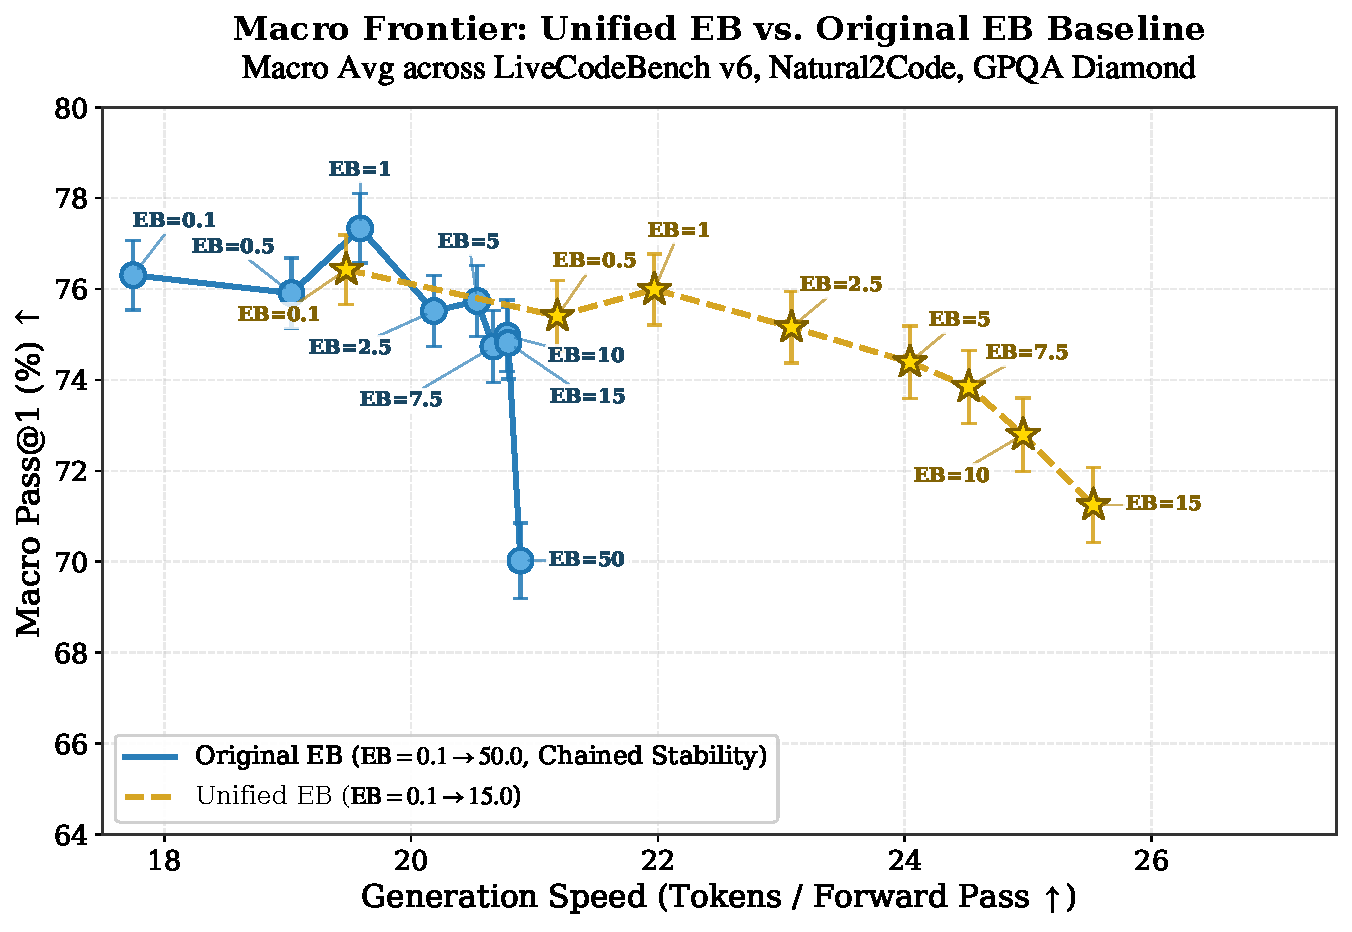
\includegraphics[width=\linewidth]{images/fig_macro_frontier_original_vs_unified.pdf}
        \caption{Original vs.\ unified stopping.}
        \label{fig:unified-vs-orig}
    \end{subfigure}
    \hfill
    \begin{subfigure}[b]{0.49\textwidth}
        \centering
        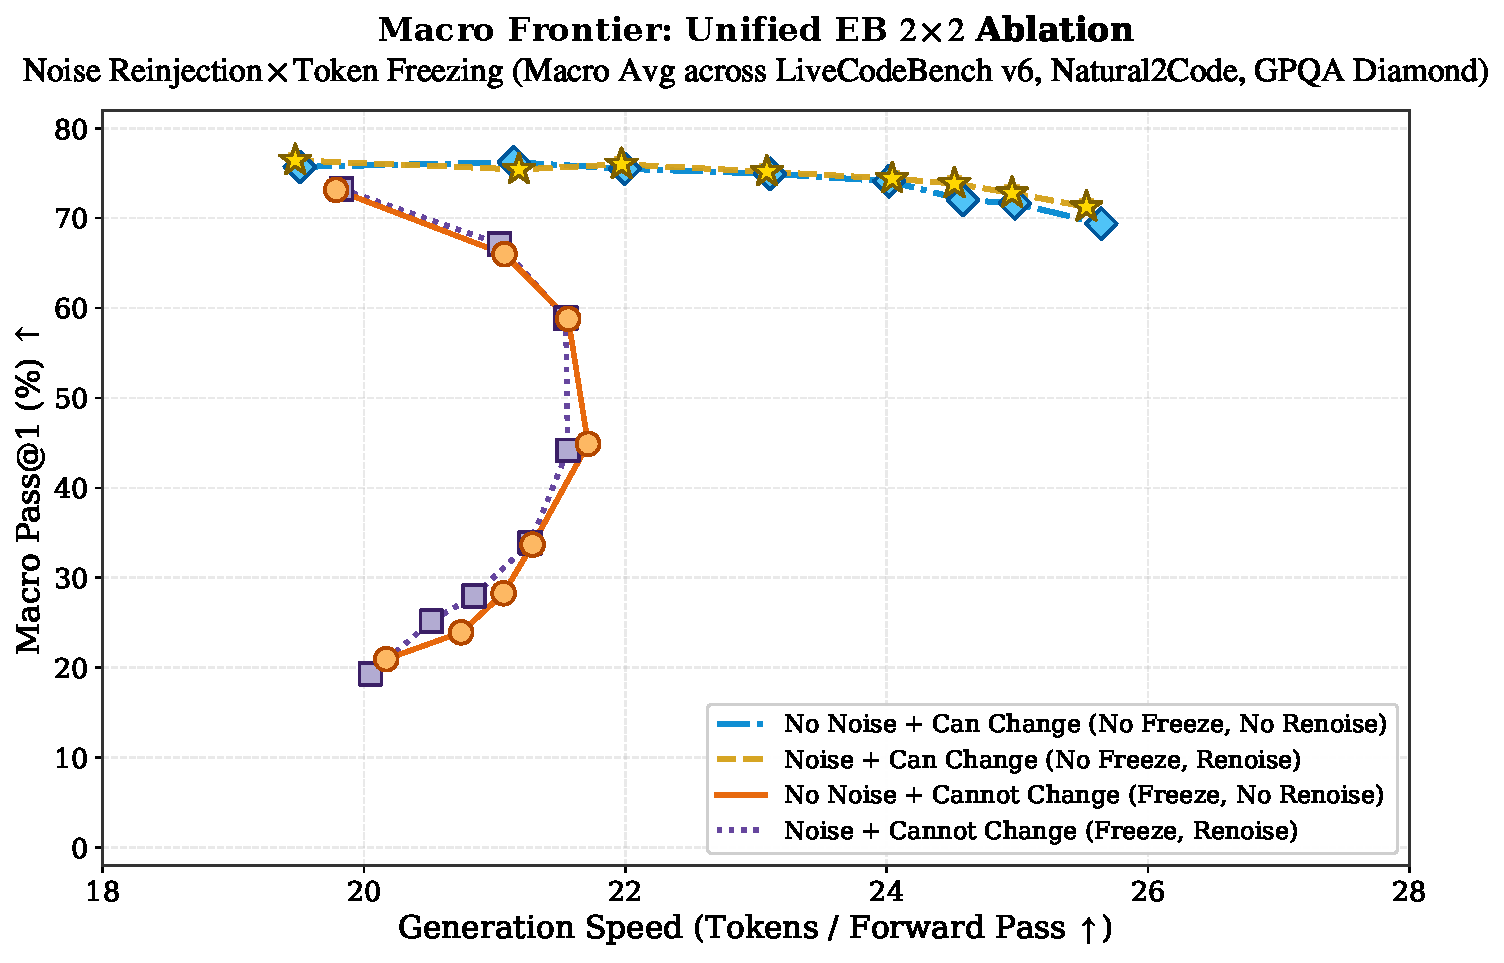
\includegraphics[width=\linewidth]{images/fig_macro_frontier_unified_ablation_2x2.pdf}
        \caption{Frozen vs.\ base EB sampler.}
        \label{fig:frozen-eb-frontier}
    \end{subfigure}

    \vspace{6pt}

    \begin{subfigure}[b]{\textwidth}
        \centering
        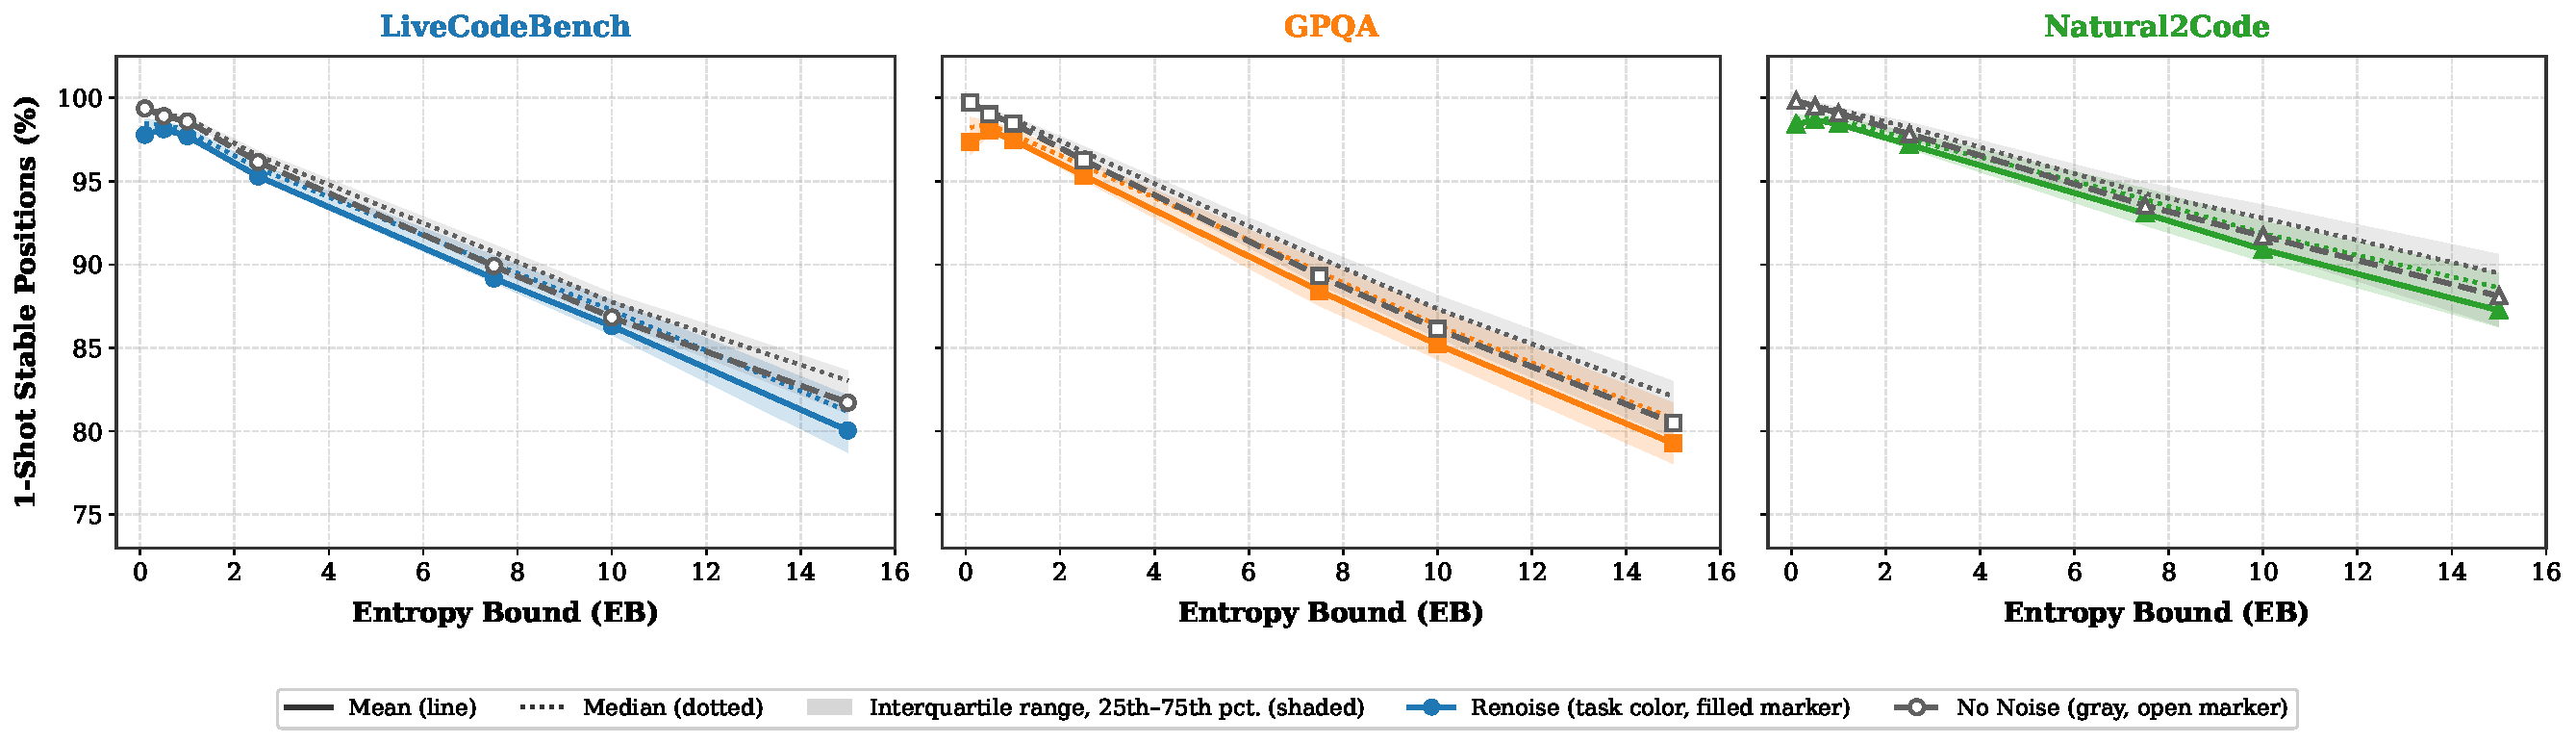
\includegraphics[width=\linewidth]{images/fig_1shot_stability_1x2_row.pdf}
        \caption{Stability of accepted tokens.}
        \label{fig:self-correct}
    \end{subfigure}
    \caption{\textbf{(a)} The unified stopping criterion matches the original at a slight speedup. \textbf{(b)} Pareto frontier of the modified EB sampler: larger entropy bounds trade performance for throughput, and the frozen variant degrades much faster than the base version, showing that the flexibility of the uniform diffusion process drives the frontier. \textbf{(c)} Accepted tokens are revised more often at higher entropy bounds (in both argmax and sampled-token stability), independent of renoising.}
    \label{fig:eb-frontiers}
\end{figure}
\paragraph{Setup}
We focus on the EB sampler, as it is the default sampler used in \citet{team2026diffusiongemma}.
Our goal is to determine if DiffusionGemma exhibits self-correcting behavior, and whether this is driven by the model or the sampler.
To do this, we measure the macro-average of AIME 2026, LCB v6, and HumanEval.
We introduce two interventions axis to investigate these questions: whether accepted tokens are "frozen" as in masked diffusion, and whether rejected tokens are renoised per the original sampler.

\paragraph{Frozen EB Sampler}
To do this, we first introduce a "freezing" variant of the EB sampler, where positions that are accepted under the EB rule cannot be changed later on, similar to masked diffusion. 
We refer to the original EB sampler as "unconstrained", as any position can be changed regardless of whether it was already accepted under the EB rule.

\paragraph{No Noise}
To determine whether the self-correction is driven by the sampler, we additionally introduce a version of the sampler that does not renoise the rejected positions as done in the original sampler. 
If there is no additional noise injection, then the model must be able to directly correct mistakes as opposed to relying on the noise to reset incorrect positions.
This can be thought of as an Euler sampler, as it is strictly interpolating between a uniform random sample and the final sample.

\paragraph{Ablation}
Both the no noise and frozen EB sampler are orthogonal directions of intervention. Thus we ablate over all four combinations and show the results in Figure \ref{fig:frozen-eb-frontier}.
For each possible combination, we do a sweep over various entropy bound values to examine how they are affected by more relaxed thresholds. 
For the unconstrained variants, we also track the empirical frequencies of each position being altered during the denoising trajectory after the initial acceptance under the EB rule.
We show these position volatility metrics in Figure \ref{fig:self-correct}.



\paragraph{Results}
We observe that for each adaptive variant, the unconstrained sampler achieves a superior pareto frontier than the frozen sampler, and this gap increases with further relaxation of the thresholds.
Furthermore, the number of positions that change after initial acceptance increases with higher entropy thresholds, and is relatively unaffected by whether the sampler uses noise injection.
This indicates that 1) the model does rely on self correction, as removing this deteriorates performance at relaxed thresholds; and 2) the self-correcion is driven by the changes in the models posterior as opposed to renoising, as removing noise does not alter post-acceptance behavior.

\subsection{Autoregressive Acceptance Order}
Here we examine the acceptance order of DiffusionGemma across a range of different acceptance rules.
We observe that DiffusionGemma exhibits a sampling order strongly biased towards autoregressive generation.
This autoregressive bias results in many denoising slots within a canvas being "wasted" on tokens that have already converged.
As a result, a form of rolling sampler where the window moves incrementally through the sequence rather than block by block becomes increasingly appealing as a way to extend the pareto frontier.

\begin{figure}[tbp]
\centering
\begin{tikzpicture}[x=0.205cm, y=0.205cm]

\definecolor{cwinfill}{HTML}{9FE1CB}
\definecolor{cwinedge}{HTML}{0F6E56}
\definecolor{camber}{HTML}{E8A13C}
\definecolor{camberedge}{HTML}{A96A0B}
\definecolor{cwaste}{HTML}{C0553C}
\definecolor{cwasteedge}{HTML}{7A2E1C}
\definecolor{cnoise}{HTML}{D3D1C7}
\definecolor{cnoiseedge}{HTML}{888780}
\definecolor{cclean}{HTML}{FFFFFF}
\definecolor{ccleanedge}{HTML}{B4B4A9}
\definecolor{cframe}{HTML}{2B5E94}

\newcommand{\gridcell}[3]{%
  \ifcase#3\relax
  \or \fill[cwinfill!65, draw=cwinedge,   line width=0.3pt, rounded corners=0.5pt] (#1, -#2) rectangle ++(0.88, -0.88);
  \or \fill[camber!45,   draw=camberedge, line width=0.3pt, rounded corners=0.5pt] (#1, -#2) rectangle ++(0.88, -0.88);
  \or \fill[cwaste,      draw=cwasteedge, line width=0.3pt, rounded corners=0.5pt] (#1, -#2) rectangle ++(0.88, -0.88);
  \or \fill[cclean,      draw=ccleanedge, line width=0.3pt, rounded corners=0.5pt] (#1, -#2) rectangle ++(0.88, -0.88);
  \or \fill[cnoise,      draw=cnoiseedge, line width=0.3pt, rounded corners=0.5pt] (#1, -#2) rectangle ++(0.88, -0.88);
  \fi}

\newcommand{\gridrow}[4]{%
  \foreach \c in {0,...,23} {%
    \pgfmathtruncatemacro{\sty}{\c<#3 ? 4 : (\c<#4 ? 1 : 5)}%
    \pgfmathsetmacro{\xpos}{\c + #1}%
    \gridcell{\xpos}{#2}{\sty}%
  }}

\newcommand{\gridmarks}[4]{%
  \foreach \c in {#4} {%
    \pgfmathsetmacro{\xpos}{\c + #1}%
    \gridcell{\xpos}{#2}{#3}%
  }}

\newcommand{\keydenoise}{\begin{tikzpicture}[baseline=-0.5ex, x=0.30cm, y=0.30cm]
  \fill[cwinfill!65, draw=cwinedge, line width=0.3pt, rounded corners=0.5pt] (0,-0.5) rectangle ++(0.88,1);
\end{tikzpicture}}
\newcommand{\keyaccept}{\begin{tikzpicture}[baseline=-0.5ex, x=0.30cm, y=0.30cm]
  \fill[camber!45, draw=camberedge, line width=0.3pt, rounded corners=0.5pt] (0,-0.5) rectangle ++(0.88,1);
\end{tikzpicture}}
\newcommand{\keywaste}{\begin{tikzpicture}[baseline=-0.5ex, x=0.30cm, y=0.30cm]
  \fill[cwaste, draw=cwasteedge, line width=0.3pt, rounded corners=0.5pt] (0,-0.5) rectangle ++(0.88,1);
\end{tikzpicture}}
\newcommand{\keycache}{\begin{tikzpicture}[baseline=-0.5ex, x=0.30cm, y=0.30cm]
  \fill[cclean, draw=ccleanedge, line width=0.3pt, rounded corners=0.5pt] (0,-0.5) rectangle ++(0.88,1);
\end{tikzpicture}}
\newcommand{\keyunadmitted}{\begin{tikzpicture}[baseline=-0.5ex, x=0.30cm, y=0.30cm]
  \fill[cnoise, draw=cnoiseedge, line width=0.3pt, rounded corners=0.5pt] (0,-0.5) rectangle ++(0.88,1);
\end{tikzpicture}}

\node[anchor=west, font=\footnotesize\bfseries] at (0, 1.5) {(a) Block sampler, $b=8$: 19 passes};

\gridrow{0}{0}{0}{8}
\gridrow{0}{1}{0}{8}
\gridrow{0}{2}{0}{8}                     \gridmarks{0}{2}{2}{0,3}
\gridrow{0}{3}{0}{8} \gridmarks{0}{3}{3}{0,3}          \gridmarks{0}{3}{2}{1,2}
\gridrow{0}{4}{0}{8} \gridmarks{0}{4}{3}{0,1,2,3}      \gridmarks{0}{4}{2}{4,6}
\gridrow{0}{5}{0}{8} \gridmarks{0}{5}{3}{0,1,2,3,4,6}  \gridmarks{0}{5}{2}{5,7}
\gridrow{0}{6}{8}{16}
\gridrow{0}{7}{8}{16}
\gridrow{0}{8}{8}{16}                        \gridmarks{0}{8}{2}{8,11}
\gridrow{0}{9}{8}{16}  \gridmarks{0}{9}{3}{8,11}             \gridmarks{0}{9}{2}{9}
\gridrow{0}{10}{8}{16} \gridmarks{0}{10}{3}{8,9,11}          \gridmarks{0}{10}{2}{10,13}
\gridrow{0}{11}{8}{16} \gridmarks{0}{11}{3}{8,9,10,11,13}    \gridmarks{0}{11}{2}{12,14}
\gridrow{0}{12}{8}{16} \gridmarks{0}{12}{3}{8,9,10,11,12,13,14} \gridmarks{0}{12}{2}{15}
\gridrow{0}{13}{16}{24}
\gridrow{0}{14}{16}{24}
\gridrow{0}{15}{16}{24}                          \gridmarks{0}{15}{2}{16,19}
\gridrow{0}{16}{16}{24} \gridmarks{0}{16}{3}{16,19}              \gridmarks{0}{16}{2}{17,18}
\gridrow{0}{17}{16}{24} \gridmarks{0}{17}{3}{16,17,18,19}        \gridmarks{0}{17}{2}{20,22}
\gridrow{0}{18}{16}{24} \gridmarks{0}{18}{3}{16,17,18,19,20,22}  \gridmarks{0}{18}{2}{21,23}

\foreach \x in {7.94, 15.94} {
  \draw[cframe, dashed, line width=0.4pt] (\x, 0.3) -- (\x, -19.2);
}
\node[anchor=east, font=\scriptsize] at (-0.5, -0.44) {$t=1$};
\node[anchor=east, font=\scriptsize] at (-0.5, -18.44) {$t=19$};

\node[anchor=west, font=\footnotesize\bfseries] at (29.5, 1.5) {(b) Rolling sampler, $w=8$: 13 passes};

\gridrow{29.5}{0}{0}{8}
\gridrow{29.5}{1}{0}{8}
\gridrow{29.5}{2}{0}{8}                          \gridmarks{29.5}{2}{2}{0,3}
\gridrow{29.5}{3}{1}{9}   \gridmarks{29.5}{3}{3}{3}          \gridmarks{29.5}{3}{2}{1,2}
\gridrow{29.5}{4}{4}{12}                         \gridmarks{29.5}{4}{2}{4,6}
\gridrow{29.5}{5}{5}{13}  \gridmarks{29.5}{5}{3}{6}          \gridmarks{29.5}{5}{2}{5,7,8}
\gridrow{29.5}{6}{9}{17}                         \gridmarks{29.5}{6}{2}{9,12}
\gridrow{29.5}{7}{10}{18} \gridmarks{29.5}{7}{3}{12}         \gridmarks{29.5}{7}{2}{10,11}
\gridrow{29.5}{8}{13}{21}                        \gridmarks{29.5}{8}{2}{13,14,17}
\gridrow{29.5}{9}{15}{23} \gridmarks{29.5}{9}{3}{17}         \gridmarks{29.5}{9}{2}{16,18}
\gridrow{29.5}{10}{15}{23} \gridmarks{29.5}{10}{3}{16,17,18} \gridmarks{29.5}{10}{2}{15,19}
\gridrow{29.5}{11}{20}{24}                       \gridmarks{29.5}{11}{2}{20,22}
\gridrow{29.5}{12}{21}{24} \gridmarks{29.5}{12}{3}{22}       \gridmarks{29.5}{12}{2}{21,23}

\node[anchor=east, font=\scriptsize] at (29.0, -0.44) {$t=1$};
\node[anchor=east, font=\scriptsize] at (29.0, -12.44) {$t=13$};

\node[anchor=north, font=\scriptsize, inner sep=0pt] at (26.7, -20.4) {%
  \begin{tabular}{@{}l@{~}l@{\hspace{1.8em}}l@{~}l@{\hspace{1.8em}}l@{~}l@{}}
    \keydenoise & denoising slot   & \keyaccept     & accepted on this pass &
    \keywaste   & wasted: re-denoised while waiting \\[2.5pt]
    \keycache   & in the KV cache  & \keyunadmitted & not yet admitted      &
                &                                    \\
  \end{tabular}};

\end{tikzpicture}
\caption{\textbf{Where the denoising slots go.} Both samplers denoise a
width-$8$ window per pass in the same order, and the colours are those of
Figure~\ref{fig:algorithm-concept}: teal = still denoising, amber = accepted
on this pass, white = already encoded and in the KV cache, gray = not yet
admitted.  Brick marks a slot spent re-denoising a position that was already
accepted but is still waiting for its prefix, that is, wasted work.
\textbf{(a)} The block sampler appends only once the block is fully resolved,
so converged positions idle and each block re-pays warm-up.  \textbf{(b)} The
rolling sampler appends the accepted prefix immediately and admits fresh
positions in its place, wasting far fewer slots.}
\label{fig:block-vs-rolling}
\end{figure}


\paragraph{Defining Redundant Computations}
Here we define what constitutes a redundant computation.
Our goal is to measure the computations that could be conceivable omitted without drastically impacting the model's behavior.
Thus we define wasted denoising slots as positions that have already converged and are part of a contiguous prefix that could be appended to the KV cache.
We illustrate this definition in Figure \ref{fig:block-vs-rolling}, against the ideal sampler that commits them to the KV cache and avoids redundant denoising steps.

\begin{figure}[tbp]
    \centering
    \begin{subfigure}[b]{\textwidth}
        \centering
        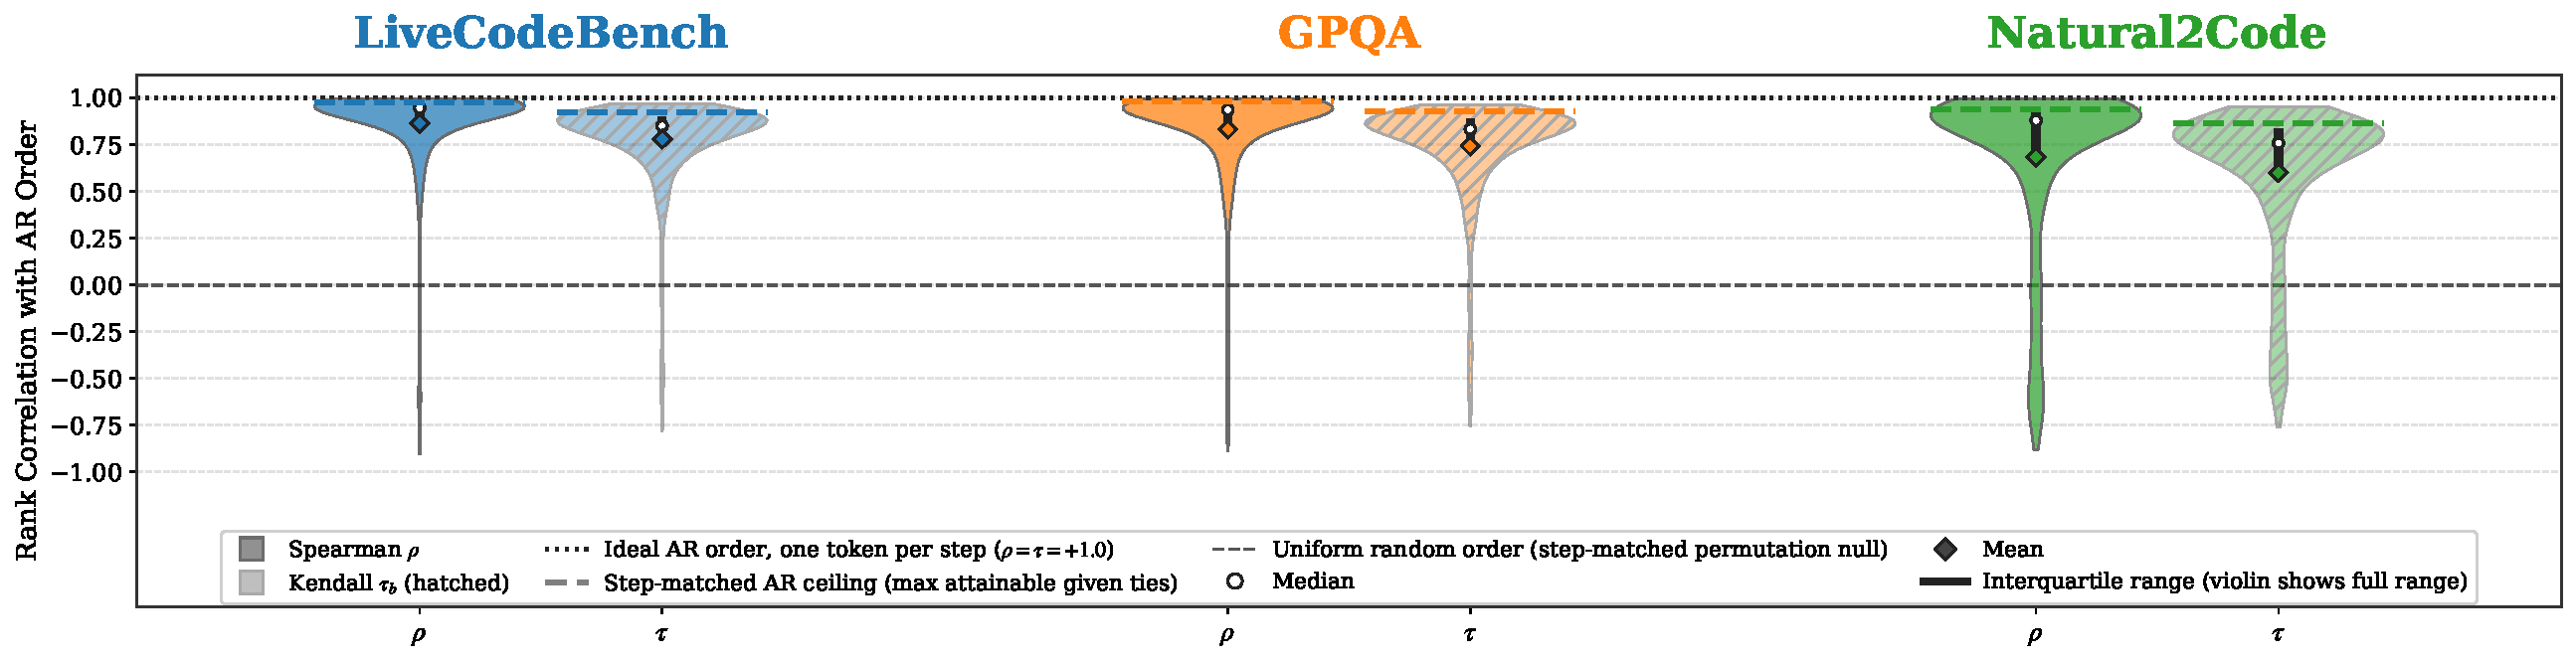
\includegraphics[width=\linewidth]{images/fig_ar_order_correlation_eb0.1_renoise.pdf}
        \caption{Commitment order vs.\ AR order.}
        \label{fig:ar-order-correlation}
    \end{subfigure}

    \vspace{6pt}

    \begin{subfigure}[b]{\textwidth}
        \centering
        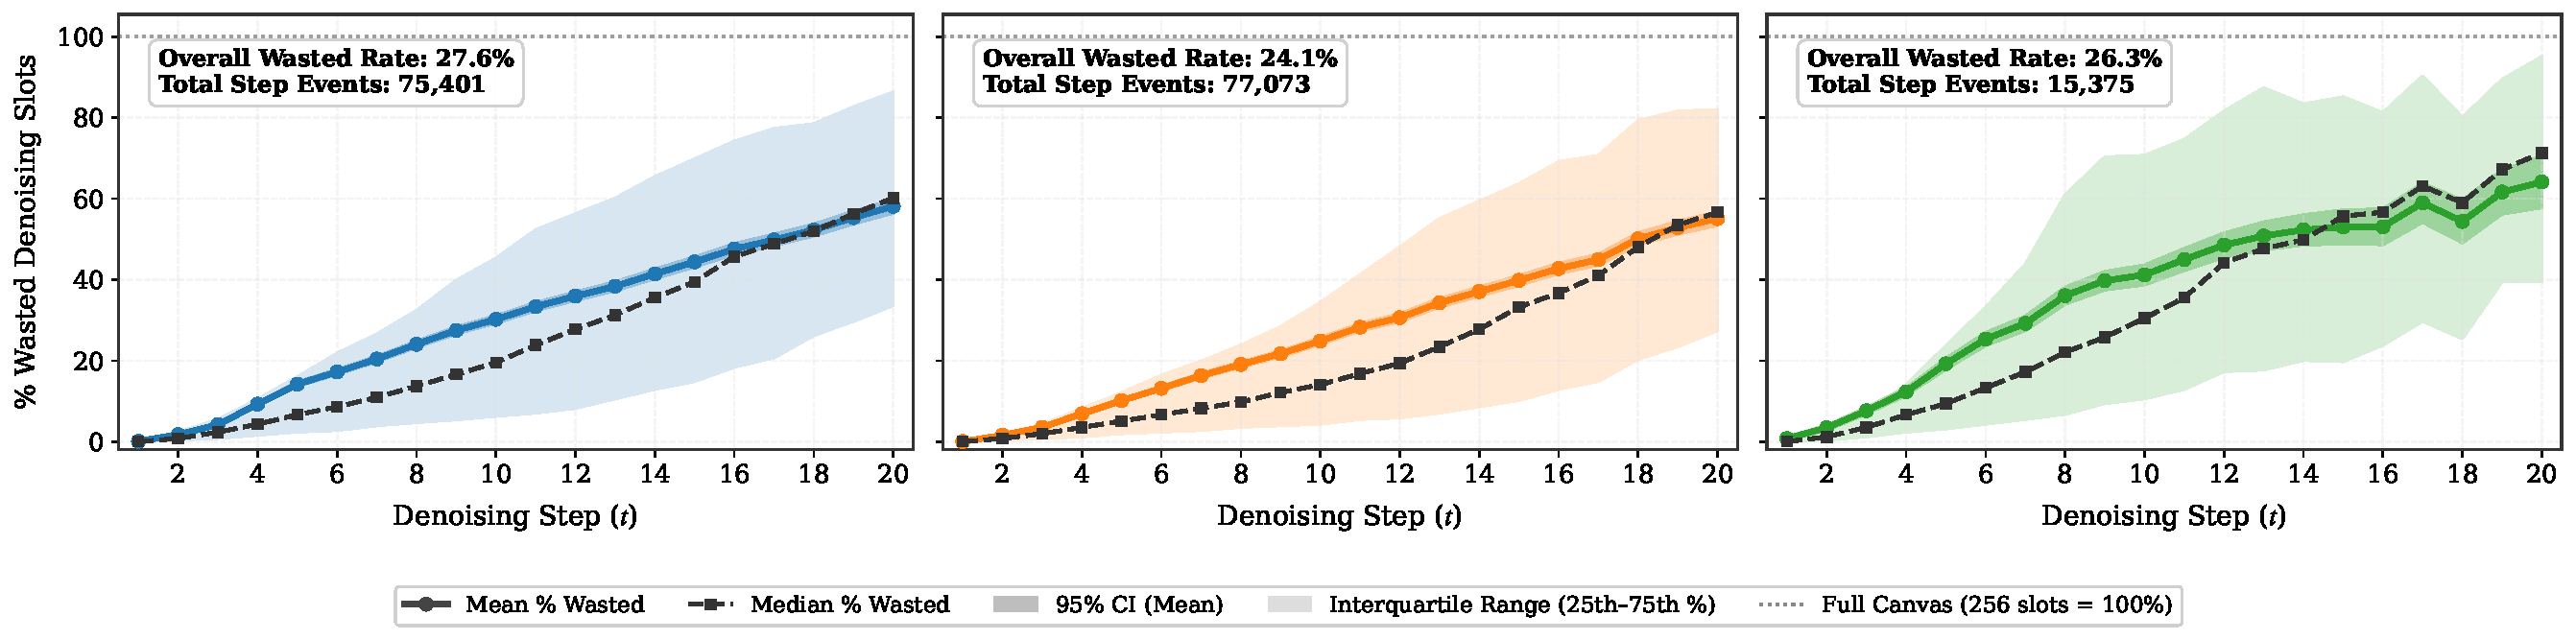
\includegraphics[width=\linewidth]{images/wasted_canvas_slots_lcb_gpqa_n2c.pdf}
        \caption{Wasted denoising slots.}
        \label{fig:wasted-slots}
    \end{subfigure}
    \caption{\textbf{(a)} Spearman $\rho$ and Kendall $\tau$ between the commitment order of the DiffusionGemma EB sampler and the AR generation order; across all tasks the sampler is strongly biased towards left-to-right order. \textbf{(b)} Number of wasted denoising slots averaged across canvases for AIME, LCB and HumanEval. For a given sampling step, a slot is wasted if it belongs to a contiguous prefix that has already converged to its final token. Past 10 denoising steps, over half of the canvas slots are wasted.}
    \label{fig:wasted}
\end{figure}

\paragraph{Experimental Setup}
We run the unified EB sampler on LCB v6, GPQA Diamond and Natural2Code. We track the trajectories of each denoising block, and consider a position as converged when it realizes the value that ends up being committed to the KV cache.

\paragraph{Results}
In Figure \ref{fig:ar-order-correlation}, we observe that the convergence orderign of positions is very correlated with left-to-right order. This explains the behavior of wasted denoising slots in Figure \ref{fig:wasted-slots}, where we observe that the percentage of wasted slots increases monotonically during the denoising trajectory.  

This has been observed previously by \citep{asaria2026neither}, where they observe the autoregressive bias of the DiffusionGemma sampler. 
This is not a model specific quirk: this aligns with many general observations of the sampling behavior for confidence-based samplers for large scale diffusion language models. 
\citet{kim2026interface} demonstrates that confidence based samplers tend to generate samples that are very similar to those produced by left-to-right autoregressive order. 
Other works demonstrate that the ordering itself is highly left to right and provide various explanations for why \citep{gong2026diffucoder, lu2026adablock, yao2026decoding}.

\paragraph{Self Correcting or Rolling?}
Through studying adaptive samplers for uniform diffusion, we observe the following:
\begin{enumerate}
    \item DiffusionGemma exhibits self correcting behavior that allows for a strictly better pareto frontier with relaxed thresholds. 
    \item DiffusionGemma also exhibits a strong autoregressive bias, which points towards a rolling mechanism as a simple means of extending the frontier.
\end{enumerate}

These two mechanisms for extending the frontier are orthogonal: self correction requires flexibility, whereas the rolling sampler would depend on token stability. 
However, it is unclear how these two orthogonal mechanisms for extending the frontier compare.
In the next section, we introduce a rolling diffusion sampler that incrementally commits tokens to the KV cache to investigate this question.

\section{\algname}
\label{sec:method}
Here we introduce \algname, a sampler designed to leverage the auto-regressive bias of DiffusionGemma to minimize redundant computations on converged tokens.
The core mechanism is straightforward: instead of waiting for the entire block to converge, we autoregressively encode and append the KV cache for any contiguous prefix of converged tokens.
We first introduce the core method, along with the pseudo-code. 
We include a diagram of the method in Figure \ref{fig:algorithm-concept}. 
\begin{figure}[tbp]
\centering
\begin{tikzpicture}[x=0.36cm, y=0.36cm]

\definecolor{cclean}{HTML}{FFFFFF}
\definecolor{ccleanedge}{HTML}{B4B4A9}
\definecolor{cwinedge}{HTML}{0F6E56}
\definecolor{cwinfill}{HTML}{9FE1CB}
\definecolor{cnoise}{HTML}{D3D1C7}
\definecolor{cnoiseedge}{HTML}{888780}
\definecolor{cframe}{HTML}{2B5E94}
\definecolor{camber}{HTML}{E8A13C}
\definecolor{camberedge}{HTML}{A96A0B}
\definecolor{mempty}{HTML}{F5F4EF}
\definecolor{memptyedge}{HTML}{C9C7BE}

\newcommand{\cellclean}[3]{%
  \fill[cclean, draw=ccleanedge, line width=0.4pt, rounded corners=1pt] (#1, #2) rectangle ++(0.9, 1);
  \node[font=\scriptsize\ttfamily, inner sep=0pt, text=black] at (#1+0.45, #2+0.5) {#3};}
\newcommand{\cellwin}[4]{%
  \fill[cwinfill!#3, draw=cwinedge, line width=0.4pt, rounded corners=1pt] (#1, #2) rectangle ++(0.9, 1);
  \node[font=\scriptsize\ttfamily, inner sep=0pt, text=black] at (#1+0.45, #2+0.5) {#4};}
\newcommand{\cellnoise}[3]{%
  \fill[cnoise, draw=cnoiseedge, line width=0.4pt, rounded corners=1pt] (#1, #2) rectangle ++(0.9, 1);
  \node[font=\scriptsize\ttfamily, inner sep=0pt, text=cnoiseedge] at (#1+0.45, #2+0.5) {#3};}
\newcommand{\cellamber}[3]{%
  \fill[camber!45, draw=camberedge, line width=0.6pt, rounded corners=1pt] (#1, #2) rectangle ++(0.9, 1);
  \node[font=\scriptsize\ttfamily, inner sep=0pt, text=black] at (#1+0.45, #2+0.5) {#3};}
\newcommand{\acceptmark}[2]{\draw[camberedge, line width=1.1pt, rounded corners=1pt] (#1+0.03, #2+0.03) rectangle ++(0.84, 0.94);}
\newcommand{\acceptdot}[2]{\fill[camberedge] (#1+0.45, #2+0.17) circle (0.12);}
\newcommand{\passframe}[2]{%
  \draw[cframe, line width=1.1pt, rounded corners=2pt, dash pattern=on 4pt off 2pt]
    (#1-0.15, #2-0.25) rectangle (#1+10.05, #2+1.25);}
\newcommand{\seqbracket}[4]{%
  \draw[line width=0.3pt] (#1, #3-0.55) -- (#1, #3-0.90) -- (#2+0.9, #3-0.90) -- (#2+0.9, #3-0.55);
  \node[font=\tiny, anchor=north, inner sep=1.5pt] at ({(#1+#2+0.9)/2}, #3-0.90) {#4};}

\newcommand{\maskpanel}[5]{%
\begin{scope}[shift={(#4cm,#5cm)}, x=0.19cm, y=0.19cm]
  \foreach \q in {#1,...,#2}{%
    \foreach \k in {#1,...,#2}{%
      \pgfmathtruncatemacro{\ii}{\k-#1}%
      \pgfmathtruncatemacro{\jj}{\q-#1}%
      \ifnum\q>#3\relax
        \ifnum\k>#3\relax
          \fill[cwinfill!65, draw=cwinedge, line width=0.25pt, rounded corners=0.4pt] (\ii,-\jj) rectangle ++(0.88,-0.88);
        \else
          \fill[camber!20, draw=camberedge, line width=0.25pt, rounded corners=0.4pt] (\ii,-\jj) rectangle ++(0.88,-0.88);
        \fi
      \else
        \ifnum\k>\q\relax
          \fill[mempty, draw=memptyedge, line width=0.25pt, rounded corners=0.4pt] (\ii,-\jj) rectangle ++(0.88,-0.88);
        \else
          \fill[camber!55, draw=camberedge, line width=0.25pt, rounded corners=0.4pt] (\ii,-\jj) rectangle ++(0.88,-0.88);
        \fi
      \fi}}%
  \pgfmathtruncatemacro{\cc}{#3-#1+1}%
  \pgfmathtruncatemacro{\nn}{#2-#1+1}%
  \ifnum\cc>0\relax
    \draw[dashed, line width=0.4pt] (\cc-0.06, 0.5) -- (\cc-0.06, -\nn-0.1);
    \draw[dashed, line width=0.4pt] (-0.5, -\cc+0.06) -- (\nn+0.1, -\cc+0.06);
    \draw[camberedge, line width=0.8pt, rounded corners=0.6pt] (-0.06, 0.06) rectangle (\cc-0.12, -\cc+0.12);
  \fi
\end{scope}}
\newcommand{\maskbrackets}[4]{%
\begin{scope}[shift={(#3cm,#4cm)}, x=0.19cm, y=0.19cm]
  \ifnum#1>0\relax
    \draw[line width=0.3pt] (0,-#2-0.5) -- (0,-#2-0.9) -- (#1-0.12,-#2-0.9) -- (#1-0.12,-#2-0.5);
    \node[font=\tiny, anchor=north, inner sep=1.5pt] at (#1/2-0.06, -#2-0.9) {prefix};
  \fi
  \draw[line width=0.3pt] (#1,-#2-0.5) -- (#1,-#2-0.9) -- (#2-0.12,-#2-0.9) -- (#2-0.12,-#2-0.5);
  \node[font=\tiny, anchor=north, inner sep=1.5pt] at ({(#1+#2)/2-0.06}, -#2-0.9) {window};
\end{scope}}

\newcommand{\keyencoded}{\begin{tikzpicture}[baseline=-0.5ex, x=0.36cm, y=0.36cm]
  \fill[cclean, draw=ccleanedge, line width=0.4pt, rounded corners=1pt] (0,-0.5) rectangle ++(0.9,1);
\end{tikzpicture}}
\newcommand{\keyaccepted}{\begin{tikzpicture}[baseline=-0.5ex, x=0.36cm, y=0.36cm]
  \fill[cwinfill!30, draw=cwinedge, line width=0.4pt, rounded corners=1pt] (0,-0.5) rectangle ++(0.9,1);
  \draw[camberedge, line width=1.1pt, rounded corners=1pt] (0.03,-0.47) rectangle ++(0.84,0.94);
\end{tikzpicture}}
\newcommand{\keywaiting}{\begin{tikzpicture}[baseline=-0.5ex, x=0.36cm, y=0.36cm]
  \fill[cwinfill!30, draw=cwinedge, line width=0.4pt, rounded corners=1pt] (0,-0.5) rectangle ++(0.9,1);
  \fill[camberedge] (0.45,-0.33) circle (0.12);
\end{tikzpicture}}
\newcommand{\keyprefix}{\begin{tikzpicture}[baseline=-0.5ex, x=0.36cm, y=0.36cm]
  \fill[camber!45, draw=camberedge, line width=0.6pt, rounded corners=1pt] (0,-0.5) rectangle ++(0.9,1);
\end{tikzpicture}}
\newcommand{\keynoise}{\begin{tikzpicture}[baseline=-0.5ex, x=0.36cm, y=0.36cm]
  \fill[cnoise, draw=cnoiseedge, line width=0.4pt, rounded corners=1pt] (0,-0.5) rectangle ++(0.9,1);
  \node[font=\scriptsize\ttfamily, inner sep=0pt, text=cnoiseedge] at (0.45,0) {k};
\end{tikzpicture}}
\newcommand{\keymcausal}{\begin{tikzpicture}[baseline=-0.5ex, x=0.36cm, y=0.36cm]
  \fill[camber!55, draw=camberedge, line width=0.4pt, rounded corners=1pt] (0,-0.5) rectangle ++(0.9,1);
\end{tikzpicture}}
\newcommand{\keymcross}{\begin{tikzpicture}[baseline=-0.5ex, x=0.36cm, y=0.36cm]
  \fill[camber!20, draw=camberedge, line width=0.4pt, rounded corners=1pt] (0,-0.5) rectangle ++(0.9,1);
\end{tikzpicture}}
\newcommand{\keymbidi}{\begin{tikzpicture}[baseline=-0.5ex, x=0.36cm, y=0.36cm]
  \fill[cwinfill!65, draw=cwinedge, line width=0.4pt, rounded corners=1pt] (0,-0.5) rectangle ++(0.9,1);
\end{tikzpicture}}
\newcommand{\keymempty}{\begin{tikzpicture}[baseline=-0.5ex, x=0.36cm, y=0.36cm]
  \fill[mempty, draw=memptyedge, line width=0.4pt, rounded corners=1pt] (0,-0.5) rectangle ++(0.9,1);
\end{tikzpicture}}

\node[anchor=east, font=\small\bfseries] at (-0.60, 0.50) {step $t$};
\cellclean{0}{0}{t}
\cellclean{1}{0}{h}
\cellclean{2}{0}{e}
\cellclean{3}{0}{}
\cellclean{4}{0}{c}
\cellclean{5}{0}{a}
\cellclean{6}{0}{t}
\cellclean{7}{0}{}
\cellwin{8}{0}{30}{m}
\cellwin{9}{0}{30}{e}
\cellwin{10}{0}{55}{r}
\cellwin{11}{0}{30}{w}
\cellwin{12}{0}{70}{s}
\cellwin{13}{0}{90}{}
\cellwin{14}{0}{100}{q}
\cellwin{15}{0}{100}{7}
\cellwin{16}{0}{100}{x}
\cellwin{17}{0}{100}{v}
\cellnoise{18}{0}{9}
\cellnoise{19}{0}{k}
\cellnoise{20}{0}{z}
\cellnoise{21}{0}{3}
\cellnoise{22}{0}{b}
\cellnoise{23}{0}{5}
\acceptmark{8}{0}
\acceptmark{9}{0}
\acceptmark{11}{0}
\passframe{8}{0}
\seqbracket{8}{17}{0}{10 positions per pass}
\maskpanel{8}{17}{7}{9.25}{1.13}

\node[font=\scriptsize, anchor=south, text=ccleanedge!60!black] at (3.95, 1.32) {KV cache};
\node[cframe, font=\scriptsize, anchor=south] at (12.95, 1.32) {processed this pass};
\node[cnoiseedge, font=\scriptsize, anchor=south] at (20.95, 1.32) {not yet admitted};
\node[font=\scriptsize, anchor=south] at (10.20cm, 1.57cm) {attention mask};
\node[font=\tiny, anchor=south] at (10.20cm, 1.19cm) {keys $\rightarrow$};
\node[font=\tiny, rotate=90, anchor=south] at (9.09cm, 0.18cm) {queries};

\node[anchor=east, font=\small\bfseries] at (-0.60, -6.50) {step $t{+}1$};
\cellclean{0}{-7.00}{t}
\cellclean{1}{-7.00}{h}
\cellclean{2}{-7.00}{e}
\cellclean{3}{-7.00}{}
\cellclean{4}{-7.00}{c}
\cellclean{5}{-7.00}{a}
\cellclean{6}{-7.00}{t}
\cellclean{7}{-7.00}{}
\cellamber{8}{-7.00}{m}
\cellamber{9}{-7.00}{e}
\cellwin{10}{-7.00}{30}{o}
\cellwin{11}{-7.00}{30}{w}
\cellwin{12}{-7.00}{30}{s}
\cellwin{13}{-7.00}{30}{}
\cellwin{14}{-7.00}{55}{l}
\cellwin{15}{-7.00}{55}{o}
\cellwin{16}{-7.00}{70}{u}
\cellwin{17}{-7.00}{70}{d}
\cellnoise{18}{-7.00}{9}
\cellnoise{19}{-7.00}{k}
\cellnoise{20}{-7.00}{z}
\cellnoise{21}{-7.00}{3}
\cellnoise{22}{-7.00}{b}
\cellnoise{23}{-7.00}{5}
\acceptmark{10}{-7.00}
\acceptdot{11}{-7.00}
\acceptmark{12}{-7.00}
\acceptmark{13}{-7.00}
\passframe{8}{-7.00}
\maskpanel{8}{17}{9}{9.25}{-1.39}

\node[anchor=east, font=\small\bfseries] at (-0.60, -13.50) {step $t{+}2$};
\cellclean{0}{-14.00}{t}
\cellclean{1}{-14.00}{h}
\cellclean{2}{-14.00}{e}
\cellclean{3}{-14.00}{}
\cellclean{4}{-14.00}{c}
\cellclean{5}{-14.00}{a}
\cellclean{6}{-14.00}{t}
\cellclean{7}{-14.00}{}
\cellclean{8}{-14.00}{m}
\cellclean{9}{-14.00}{e}
\cellamber{10}{-14.00}{o}
\cellamber{11}{-14.00}{w}
\cellamber{12}{-14.00}{s}
\cellamber{13}{-14.00}{}
\cellwin{14}{-14.00}{30}{l}
\cellwin{15}{-14.00}{30}{o}
\cellwin{16}{-14.00}{30}{u}
\cellwin{17}{-14.00}{30}{d}
\cellwin{18}{-14.00}{100}{9}
\cellwin{19}{-14.00}{100}{k}
\cellnoise{20}{-14.00}{z}
\cellnoise{21}{-14.00}{3}
\cellnoise{22}{-14.00}{b}
\cellnoise{23}{-14.00}{5}
\acceptmark{14}{-14.00}
\acceptmark{15}{-14.00}
\acceptmark{16}{-14.00}
\acceptmark{17}{-14.00}
\passframe{10}{-14.00}
\seqbracket{10}{13}{-14.00}{encoded prefix}
\seqbracket{14}{19}{-14.00}{denoising window}
\maskpanel{10}{19}{13}{9.25}{-3.91}
\maskbrackets{4}{10}{9.25}{-3.91}

\node[anchor=north, font=\scriptsize, inner sep=0pt] at (5.10cm, -6.60cm) {%
  \begin{tabular}{@{}l@{~}l@{\hspace{2.2em}}l@{~}l@{}}
    \keyencoded  & already encoded, in the KV cache   & \keymcausal & prefix $\to$ prefix (causal) \\[2.5pt]
    \keyprefix   & committed, encoded on this pass    & \keymcross  & window $\to$ prefix \\[2.5pt]
    \keyaccepted & accepted on this pass              & \keymbidi   & window $\leftrightarrow$ window (bidirectional) \\[2.5pt]
    \keywaiting  & accepted earlier, awaiting prefix  & \keymempty  & masked out \\[2.5pt]
    \keynoise    & not yet admitted (noise token)     &             & \\
  \end{tabular}};

\end{tikzpicture}
\caption{Three passes of the rolling sampler.  Every pass spends a fixed
budget of ten positions (dashed frame), split between an \emph{encoded
prefix} of the tokens committed on the previous pass and the remaining
\emph{denoising window}; the mask panel on the right is exactly that block of
ten.  \textbf{Left:} positions keep their column, so each slot can be read down
its column.  Out-of-order acceptances wait for a contiguous prefix (\texttt{w}
at $t$) and unaccepted slots stay mutable (column ten: \texttt{r} $\to$
\texttt{o}).  The prefix completing at $t{+}1$ is four slots long, so four
slots must be encoded at $t{+}2$: the block advances by however many positions
graduated into the KV cache, and the split is $0{+}10$, then $2{+}8$, then
$4{+}6$.  \textbf{Right:} rows are queries, columns are keys; a coloured cell
means the query attends to the key.  The encoded prefix is causal, so its
KV-cache entries depend only on committed tokens and are never revised, while
denoising positions are bidirectional among themselves and attend fully to the
prefix.  Committing more positions per pass therefore moves the KV cache forward
faster, but leaves fewer positions to denoise on the next pass.  Every query additionally attends to the
whole KV cache (white cells), which the panels omit for space.}
\label{fig:algorithm-concept}
\end{figure}


\paragraph{Extending Adaptive Samplers}
In general, we can interpret rolling samplers as a natural extension of adaptive samplers: in addition to defining functions that map into the accept-stay-noise simplex, rolling samplers also specify $F_{commit}$.

\algname can be interpreted as an extension of the block EB sampler used in DiffusionGemma.
Rather than applying the entropy bound criterion solely to determine whether a prediction should be accepted or not, we also use it to determine whether commit to a contiguous prefix to the KV cache.
The entropy bound criterion serves as a means to accept tokens that are simultaneously highly confident and uncorrelated with each other, as \eqref{eq:eb-bound} bounds the error incurred from factorized sampling \citep{ben2026accelerated}.
Thus we used the EB criterion to define $F_{commit}$ as well as $F_{trans}$.

% Prepare the two results figures before Figure 7, preserving reference numbers.
\newsavebox{\resultspanels}
\begin{lrbox}{\resultspanels}
\begin{minipage}{\textwidth}
\captionsetup{hypcap=false}
\centering
\begin{minipage}[c]{0.49\textwidth}
\footnotesize
\setlength{\tabcolsep}{2pt}
\renewcommand{\arraystretch}{1.0}
\centering
\captionsetup{font=footnotesize}
\captionof{table}{Comparison of \textbf{EB Unified} vs.\ \textbf{Rolling} across benchmarks ($\text{EB}=0.1, \text{max\_dns}=48$). Scores report \textbf{Avg@20} $\pm$ 95\% CI (Pass@1 averaged across 20 seeds; 5 seeds for LiveCodeBench). Relative TPF deltas are shown underneath.}
\label{tab:eb_unified_vs_rolling}
\vspace{4pt}
\begin{tabular*}{\linewidth}{@{\extracolsep{\fill}}lcccc@{}}
\toprule
& \multicolumn{2}{c}{\textbf{EB Unified}} & \multicolumn{2}{c}{\textbf{Rolling}} \\
\cmidrule(lr){2-3} \cmidrule(lr){4-5}
\textbf{Task} & \textbf{Avg@20} & \textbf{TPF} & \textbf{Avg@20} & \textbf{TPF} \\
\midrule
LiveCodeBench & \begin{tabular}[t]{@{}c@{}}65.4\% \\ \scriptsize{($\pm$3.2\%)}\end{tabular} & 18.7 & \begin{tabular}[t]{@{}c@{}}62.6\% \\ \scriptsize{($\pm$3.2\%)}\end{tabular} & \begin{tabular}[t]{@{}c@{}}\textbf{26.3} \\ \scriptsize{(+40.6\%)}\end{tabular} \\
\addlinespace[2pt]
Natural2Code & \begin{tabular}[t]{@{}c@{}}\textbf{93.0\%} \\ \scriptsize{\textbf{($\pm$0.8\%)}}\end{tabular} & 22.9 & \begin{tabular}[t]{@{}c@{}}91.3\% \\ \scriptsize{($\pm$0.9\%)}\end{tabular} & \begin{tabular}[t]{@{}c@{}}\textbf{30.1} \\ \scriptsize{(+31.7\%)}\end{tabular} \\
\addlinespace[2pt]
GPQA Diamond & \begin{tabular}[t]{@{}c@{}}67.5\% \\ \scriptsize{($\pm$1.5\%)}\end{tabular} & 16.6 & \begin{tabular}[t]{@{}c@{}}68.3\% \\ \scriptsize{($\pm$1.4\%)}\end{tabular} & \begin{tabular}[t]{@{}c@{}}\textbf{23.8} \\ \scriptsize{(+43.1\%)}\end{tabular} \\
\addlinespace[2pt]
HiddenMath   & \begin{tabular}[t]{@{}c@{}}\textbf{73.9\%} \\ \scriptsize{\textbf{($\pm$0.9\%)}}\end{tabular} & 22.1 & \begin{tabular}[t]{@{}c@{}}72.6\% \\ \scriptsize{($\pm$0.9\%)}\end{tabular} & \begin{tabular}[t]{@{}c@{}}\textbf{27.2} \\ \scriptsize{(+23.2\%)}\end{tabular} \\
\addlinespace[2pt]
GSM8k        & \begin{tabular}[t]{@{}c@{}}\textbf{92.1\%} \\ \scriptsize{\textbf{($\pm$0.3\%)}}\end{tabular} & 21.7 & \begin{tabular}[t]{@{}c@{}}91.6\% \\ \scriptsize{($\pm$0.3\%)}\end{tabular} & \begin{tabular}[t]{@{}c@{}}\textbf{27.7} \\ \scriptsize{(+28.0\%)}\end{tabular} \\
\addlinespace[2pt]
IFEval       & \begin{tabular}[t]{@{}c@{}}\textbf{93.1\%} \\ \scriptsize{\textbf{($\pm$0.5\%)}}\end{tabular} & 16.8 & \begin{tabular}[t]{@{}c@{}}82.4\% \\ \scriptsize{($\pm$0.7\%)}\end{tabular} & \begin{tabular}[t]{@{}c@{}}\textbf{22.6} \\ \scriptsize{(+34.4\%)}\end{tabular} \\
\addlinespace[2pt]
MMLU         & \begin{tabular}[t]{@{}c@{}}80.3\% \\ \scriptsize{($\pm$0.4\%)}\end{tabular} & 16.2 & \begin{tabular}[t]{@{}c@{}}\textbf{82.8\%} \\ \scriptsize{\textbf{($\pm$0.4\%)}}\end{tabular} & \begin{tabular}[t]{@{}c@{}}\textbf{21.0} \\ \scriptsize{(+30.0\%)}\end{tabular} \\
\midrule
\textbf{Macro Average} & \begin{tabular}[t]{@{}c@{}}\textbf{80.7\%} \\ \scriptsize{\textbf{($\pm$0.5\%)}}\end{tabular} & 19.3 & \begin{tabular}[t]{@{}c@{}}78.8\% \\ \scriptsize{($\pm$0.5\%)}\end{tabular} & \begin{tabular}[t]{@{}c@{}}\textbf{25.5} \\ \scriptsize{\textbf{(+32.5\%)}}\end{tabular} \\
\bottomrule
\end{tabular*}



\end{minipage}\hfill
\begin{minipage}[c]{0.49\textwidth}
\centering
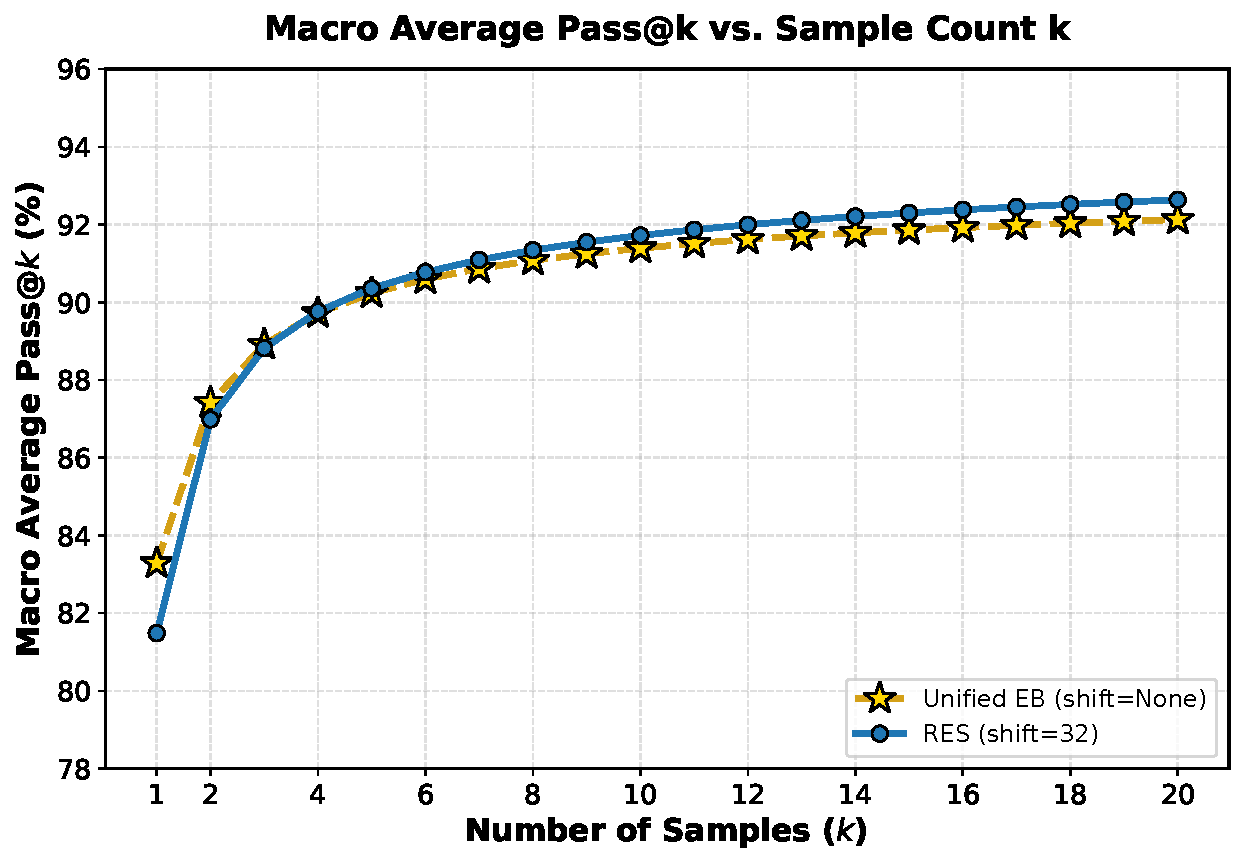
\includegraphics[width=\linewidth]{images/fig_macro_pass_at_k.pdf}
\captionof{figure}{\textbf{Macro Average Pass@$k$ vs.\ Sample Count $k$}. While EB Unified achieves higher Pass@1, Rolling ($\text{shift}=32$) exhibits stronger multi-sample scaling, overtaking EB Unified at $k \ge 6$ to reach $93.58\%$ Pass@20 while running $+31.3\%$ faster.}
\label{fig:macro_pass_at_k}

\end{minipage}
\par\vspace{12pt}
\begin{minipage}{\textwidth}
\centering
    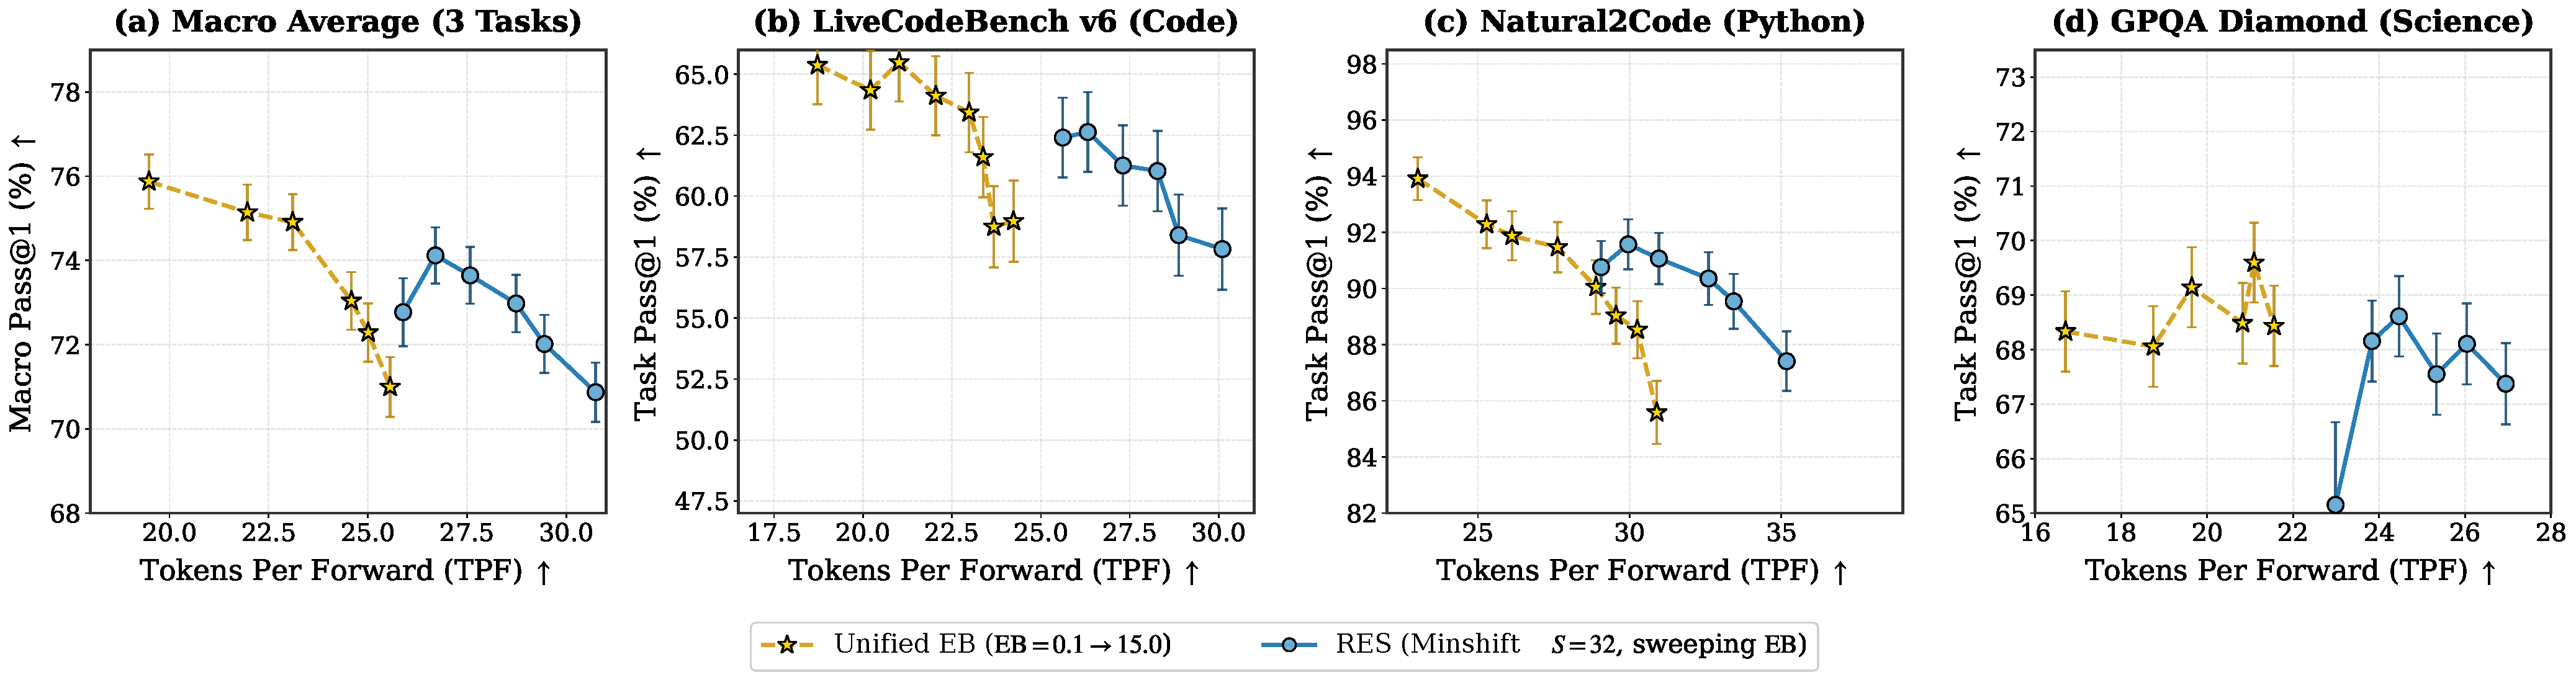
\includegraphics[width=\linewidth]{images/fig_merged_minshift32_eb01_1x4_row.pdf}
    \captionof{figure}{Comparison of Pareto frontiers between rolling sampler with minimum shift 32 and varied EB bounds $.05 \to 1.0$ for LCB v6 and Natural2Code with 5 seed averages, and GPQA Diamond with 20 seed averages due to high noise in the eval.}
    \label{fig:minshift-16}

\end{minipage}
\end{minipage}
\end{lrbox}

\Needspace{19\baselineskip}
\begin{wrapfigure}{r}{0.48\textwidth}
\captionsetup{font=footnotesize}
    \centering
    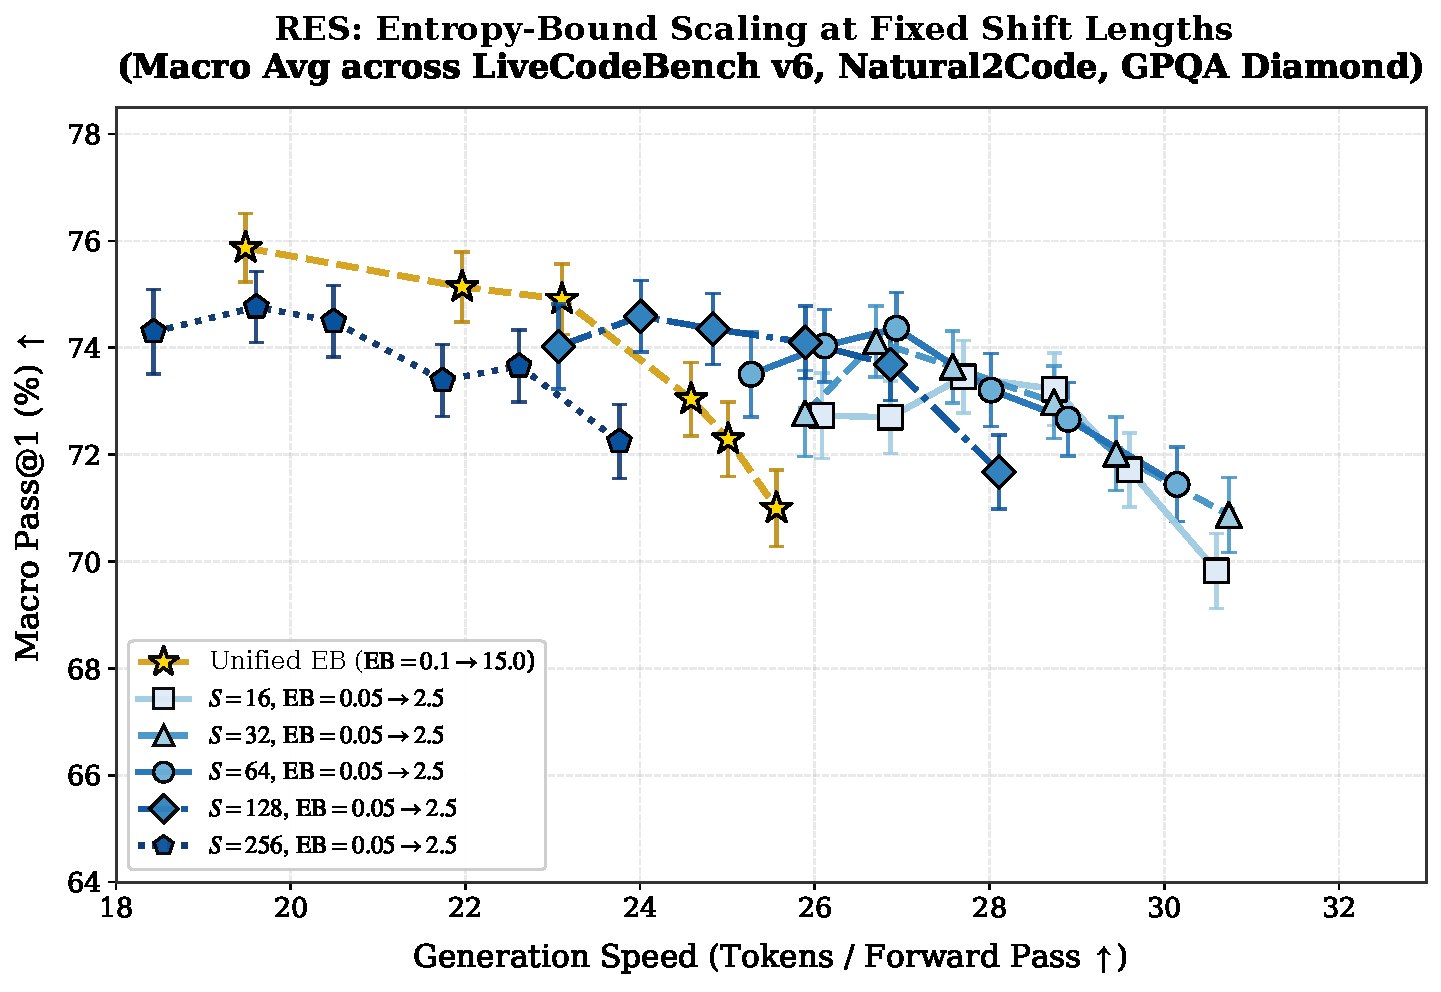
\includegraphics[width=\linewidth]{images/fig_merged_minshift_by_eb_macro.pdf}
    \caption{Generated frontiers obtained by ablating both minimum shift for $F_{commit}$ and entropy bound criterion in $F_{trans}$ for rolling sampler. We observe that the rolling optimization provides a new way to smoothly trade off performance v.s speed.}
    \label{fig:dual-frontier}
\end{wrapfigure}

\paragraph{Minimum Shift Criterion}
In order to enable smooth interpolation between the original block EB sampler and \algname, we introduce a minimum shift criterion: the contiguous prefix must at least contain the minimum shift value $m$ tokens in order to be appended to the KV cache. We find that allows for another axis for trading off performance for speed: by decreasing $m$, it is possible to accelerate the rolling sampler without altering the entropy bound. 
Furthermore, such a minimum shift criterion aligns with our desirata for tokens ready to commit to the KV cache: we would want them to be highly confident and uncorrelated with other tokens, as being correlated with other tokens means that the token could potentially change based on future fluctuations.When $m=B$, we recover the original unified EB sampler, assuming the same temperature schedule.
\input{method/attention_mask}

\paragraph{Position-based Temperature Schedule}
One natural consequence of the autoregressive bias of DiffusionGemma is that a token's position in the rolling canvas directly corresponds to how close it is to having converged. 
Thus we can modify the standard temperature shaping applied in DiffusionGemma to be based on position rather than noise level. 
This accelerates tokens that are close to the prefix, as these are closer to being committed, while allowing for positions in the suffix to explore candidate tokens.

\paragraph{Simultaneous Encoding and Denoising}
One other advantage of the rolling sampler is that the number of tokens appended to the KV cache is much smaller than the total canvas. This allows for merging both the encoding step and the denoising step present in DiffusionGemma. 
More specifically, given a window of $B$ positions and a contiguous prefix of $m$ accepted tokens, we use a causal mask for positions $0$ to $m-1$, while positions $m$ to $B-1$ have bidirectional attention.
This keeps the per forward cost the same between the original DiffusionGemma sampler and the rolling sampler, while ensuring that every step is performing denoising. 
We include a visualization of how the attention mask changes alongside the steps of the rolling sampler in Figure \ref{fig:algorithm-concept}. 

\paragraph{Any-time Sampling}
While the unified EB sampler is highly adaptive, the temperature schedule is tied to the maximum DNS, which is a hyper-parameter that must be set. 
Ideally, the maximum DNS would only serve a time-out function to prevent sampler stalls, as opposed to controlling the logit shaping.
One consequence of adopting the position-based temperature schedule is that the logit shaping becomes independent of the maximum number of DNS, making it an \textit{any-time sampler}: the maximum denoising steps serves as the maximum budget possible rather than controlling fundamental sampler behavior.

\section{Related Works}
\label{sec:adjacentworks}
Here we discuss works that are closely related to the framework and sampler modifications proposed in this work.

\subsection{Adaptive Block Samplers}
Our work is not the first to suggest incrementally moving the denoising window: \citet{luo2026dsb} applies this to masked diffusion and sees performance gains. \citet{gat2025set, arriola2025blockdiffusioninterpolatingautoregressive}.
\citet{gat2025set} fine-tunes an auto-regressive model to simultaneously decode the masked tokens ahead using the \citet{ben2026accelerated} while generating the next token auto-regressively, which is the same core idea of a rolling denoising window.
Furthermore, the denoising window is entirely defined by the entropy bound, which has been already defined in \citet{ben2026accelerated} and used in the original sampler of \citet{team2026diffusiongemma}.

Similar ideas of combining diffusion with the left-to-right bias of language have appeared even earlier, such as in \citep{wu2023ar}.
The purpose of this work isn't to introduce a novel concept, but to show how various aspects of discrete diffusion samplers can be synthesized into one simple framework to enable further flexibility in terms of the tradeoff between performance and speed.

\subsection{Rolling Diffusion Beyond Text}
Beyond text generation, the idea of rolling diffusion has been studied extensively in other domains.
Within video generation, rolling diffusion was a natural mechanism to address the temporal nature of video generation and avoid performing diffusion on every frame simultaneously \citep{ruhe2024rolling}. 
Many other works include similar mechanisms \citep{chen2024diffusion, song2025history, xie2025progressive}.

Similarly, \citet{papa2026asyncpatch} applies a similar idea to the image domain, where different patches are assigned varying levels of corruption.


\section{Experiments}
\label{sec:experiments}
\subsection{Main Results}
Here we compare the performance of the rolling sampler against the Unified EB sampler. We compare across a wide range of evaluations, and take the average performance across 20 seeds. 
We show the results in Table \ref{tab:eb_unified_vs_rolling} along with the Pass at K in Figure \ref{fig:macro_pass_at_k}.

\paragraph{Performance and Efficiency}
We observe that the rolling sampler is able to \textbf{improve algorithmic efficiency by over $30\%$} while incurring only $<3\%$ performance degradation.
We view such performance degradation as inevitable due to the exposure bias incurred when using the rolling sampler: the rolling sampler induces a noise schedule that is heavily left-to-right, which is distinct from the homogeneous noise schedule used within the block at training time.

\paragraph{Pass @ k}
We also observe that the rolling sampler exhibits larger gains with pass at k relative to the original EB sampler.
We hypothesize that the EB sampler avoids making "difficult" decisions as the sampler always accepts the lowest entropy positions first.
In contrast, the rolling mechanism along with the position-based noise schedule enforces a left-to-right generation bias, which was shown in \citet{ni2026flexibility} to improve diversity across generations. 



\subsection{Ablations}
Here we include ablation results, using the macro-average across LCB v6, GPQA Diamond, and Natural2Code.

\begin{figure}[tbp]
\centering
\usebox{\resultspanels}
\end{figure}


\paragraph{Entropy-Bound Sweep}
We sweep the entropy bound for the rolling sampler with minimum shift 32 and the unified EB sampler across LCB v6, GPQA Diamond, and Natural2Code.
We include the frontiers in Figure \ref{fig:minshift-16}.
We observe that the rolling sampler achieves a competitive frontier with the unified EB sampler, and in some cases achieves a superior frontier in terms of performance v.s efficiency. 

\paragraph{Minimum Shift Sweep}
While the unified entropy bound sampler provides one axis to trade off performance and speed, we find that the rolling sampler allows for using the minimum shift hyper-parameter in addition to the standard entropy-bound. 
In Figure \ref{fig:dual-frontier}, we observe that the rolling sampler can trade performance for speed either through the entropy bound or the minimum shift. 
Increasing the minimum shift improves performance at the expense of speed; similar to the effect of decreasing the entropy bound.
This makes sense, as the primary purpose of the minimum shift is to force the model to spend more time denoising on the current span of text in the denoising window.


\section{Conclusion}
In this work, we discuss a generic framework for discussing adaptive samplers for discrete diffusion language models.
We show how various approaches can be viewed as different answers to the same core questions: what tokens should each position realize at a given step; and when should each position be moved from the denoising window to the KV cache.
By investigating the DiffusionGemma model along the design axis exposed by this framework, we introduce a simple rolling optimization that improves the Pareto frontier between performance and efficiency.
We hope that this serves as a reasonable baseline for future improved diffusion samplers.
\FloatBarrier
\begingroup
\small
\setlength{\bibsep}{4pt}
\setlength{\parskip}{0pt}
\bibliography{iclr2025_conference}
\bibliographystyle{iclr2025_conference}
\endgroup

\clearpage
\appendix
\section{Appendix}

\subsection{Unified Stopping Criterion Relation to Original Threshold}
\label{app:unified-connection}
Here we discuss the connection between the unified stopping criterion and the original adaptive stopping mechanism originally used in \citet{team2026diffusiongemma}.



\subsection{Computation of Order Statistics}
\label{app:order-stats}
Here we provide details on how the order statistics in Figure \ref{fig:ar-order-correlation} are calculated. 

\paragraph{Acceptance Event}
To track the ordering for the unified EB sampler, we look at the first
acceptance per position, as the standard entropy bound of $0.1$ results in
positions rarely changing after the first acceptance. Concretely, for a
canvas of $b$ positions $X_1,\dots,X_b$ denoised over $T$ steps, we record
for each position the step at which it is first accepted,
\begin{equation}
  c_i \;=\; \min\bigl\{\, t \in \{1,\dots,T\} \;:\; X_i \text{ is accepted at step } t \,\bigr\},
\end{equation}
setting $c_i = T$ for the rare positions never accepted. Each generated
canvas therefore yields a commit-step vector $c \in \{1,\dots,T\}^{b}$. A
purely autoregressive sampler would produce $c_i = i$, so we measure how
closely $c$ tracks the left-to-right index.

\paragraph{Resolving Ties}
Since our goal is to compare the ranking of positions based on commitment
step, there must be a way to resolve the ties between tokens that are
accepted on the same step. To resolve this, we take the approach of
averaging the order ranking across slots that are tied, assigning each
position the fractional midrank
\begin{equation}
  r_i \;=\; \bigl|\{\,k : c_k < c_i\,\}\bigr|
        \;+\; \tfrac{1}{2}\bigl(1 + \bigl|\{\,k : c_k = c_i\,\}\bigr|\bigr).
\end{equation}
Given the list of commit steps $c = [1, 3, 1, 2, 3, 3]$, we first sort them
in ascending order, $[1, 1, 2, 3, 3, 3]$. The positions committed on the
first step occupy the first and second ranking slots, so both are assigned
the average rank $1.5$; likewise the three positions committed on the third
step occupy slots four through six and are each assigned $5$. Returning
these ranks to their original positions yields
$r = [1.5,\, 5,\, 1.5,\, 3,\, 5,\, 5]$. Averaging within tie groups keeps
tied positions exchangeable, so the statistic does not depend on an
arbitrary tie-breaking order, and preserves the rank sum
$\sum_i r_i = b(b+1)/2$.

\paragraph{Spearman $\rho$}
Given the vector of rankings, we compare it against the standard
left-to-right rankings $[1, 2, \dots, b-1, b]$ and take the Pearson
correlation coefficient to be the Spearman rank correlation $\rho$. Writing
$\pi_i = i$ for the reference ranking,
\begin{equation}
  \rho \;=\;
  \frac{\sum_{i=1}^{b} (\pi_i - \bar{\pi})(r_i - \bar{r})}
       {\sqrt{\sum_{i=1}^{b} (\pi_i - \bar{\pi})^{2}}\;
        \sqrt{\sum_{i=1}^{b} (r_i - \bar{r})^{2}}},
  \qquad \bar{\pi} = \bar{r} = \frac{b+1}{2}.
\end{equation}
We use this general form rather than the familiar
$1 - 6\sum_i d_i^{2}/\bigl(b(b^{2}-1)\bigr)$, which is valid only when the
ranks are untied.

\paragraph{Kendall $\tau$}
Spearman rank correlation may not reflect the true behavior, as it is
quadratic in terms of the differences per position. Thus we also calculate
the Kendall $\tau$, as it counts inversions and is thus less sensitive to
large differences. More specifically, for every position pair $(X_i, X_j)$
with $i < j$, the pair is \emph{concordant} if $X_i$ was committed earlier
than $X_j$, \emph{discordant} if $X_j$ was committed earlier, and
\emph{tied} if both were committed on the same step. Over all
$n_0 = \binom{b}{2}$ pairs we count
\begin{equation}
  n_c = \bigl|\{(i,j) : i<j,\; c_i < c_j\}\bigr|, \quad
  n_d = \bigl|\{(i,j) : i<j,\; c_i > c_j\}\bigr|, \quad
  n_t = n_0 - n_c - n_d .
\end{equation}
Because the reference ranking is strictly increasing, it contributes no
ties of its own, and every tied pair is tied in commit step. We report the
tie-corrected $\tau_b$, which normalises by the pairs whose order is
resolvable at all,
\begin{equation}
  \tau_b \;=\; \frac{n_c - n_d}{\sqrt{n_0\,(n_0 - n_2)}},
  \qquad
  n_2 \;=\; \sum_{s=1}^{T} \binom{m_s}{2},
\end{equation}
where $m_s$ is the number of positions first accepted at step $s$. We
additionally report the pairwise left-to-right agreement rate, which counts
ties as half-agreements,
\begin{equation}
  P_{\mathrm{l2r}} \;=\; \frac{n_c + \tfrac{1}{2} n_t}{n_0},
\end{equation}
equal to $50\%$ under a random commit order and $100\%$ under a purely
left-to-right one.

\paragraph{KDE Estimate}
To get the shape of the distribution, we use the default KDE estimator in matplotlib. 

% \begin{figure}
    \centering
    \includegraphics[width=\linewidth]{images/fig6_first_acceptance_position_scatter.pdf}
    \caption{Scatter plot showing the first accept in the trajectory (y axis) against the position within the canvas (x axis) for both tokens that realize their final identity immediately (top row) v.s tokens that fluctuate between the first acceptance and the final canvas (bottom row).}
    \label{fig:acc_vs_pos}
\end{figure}
% \begin{figure}
    \centering
    \includegraphics[width=\linewidth]{images/fig4_first_acceptance_realization.pdf}
    \caption{Histogram of behavior of positions after first acceptance in EB rule. While the majority of the positions stay the same after their first acceptance, a non trivial amount do change from the initially accepted token. This introduces the potential for performance deterioration.}
    \label{fig:placeholder}
\end{figure}
% \begin{figure}
    \centering
    \includegraphics[width=\linewidth]{images/fig5_first_acceptance_timing_histogram.pdf}
    \caption{Histogram of when the first acceptance for tokens tends to occur in the denoising trajectory, organized by tokens that realize their final token identity by the first acceptance (top row) and tokens that change (bottom row). As visible, both tend to overlap very heavily, meaning that there is no clear heuristic to distinguish between whether a position has changed to its final identity or a transient state.}
    \label{fig:acc_vs_timing}
\end{figure}
\end{document}
